% !TEX encoding = UTF-8 Unicode
\documentclass[a4paper,twocolumn,twoside]{article}
%%%%%%%%%%%%%%%%%%%%%%%%%%%%%%%%%%%%%%%%%%%%%%%%%%%%%%%%%%%%%%%%%%%
% Packages using
%%%%%%%%%%%%%%%%%%%%%%%%%%%%%%%%%%%%%%%%%%%%%%%%%%%%%%%%%%%%%%%%%%%
\ifx\pdfoutput\undefined
	\usepackage[dvips]{graphicx}
	\DeclareGraphicsExtensions{.eps}
\else
	\usepackage[pdftex]{graphicx}
	\DeclareGraphicsExtensions{.pdf,.jpg,.png,.mps}
	\pdfcompresslevel=9
\fi
\graphicspath{{./Figures_for_report/}}
\usepackage[utf8]{inputenc}
\usepackage[english]{babel}
\usepackage{indentfirst}
\addtolength{\topmargin}{-20mm}
\addtolength{\textheight}{10mm}
\usepackage{amsmath} % Added to get modern math environments
\usepackage{amssymb,amsfonts} %Added to get math
\usepackage{amsthm} % Added to get theorems
\usepackage{natbib} % Added to get better bibliography
\usepackage{soul} %underline
\usepackage{url}
%\usepackage{listings}
%\usepackage{color}
% Special hack below to break the URL!
\def\UrlBreaks{\do\.\do\@\do\\\do\/\do\!\do\_\do\|\do\;\do\>\do\]%
 \do\)\do\,\do\?\do\'\do+\do\=\do\#\do\i\do\m\do\t\do\a\do\x}%
\urlstyle{rm} %
\usepackage[bookmarks=true,bookmarksnumbered=true,hypertexnames=true,breaklinks=true,colorlinks=true]{hyperref}
\hypersetup{
pdfauthor = {Torbj\"{o}rn E. M. Nordling},
pdftitle = {Information Retrieval and Processing--Setup of a Full Text System Implementing Automatic Metadata Extraction and Visualization},
pdfsubject = {Technical Report},
pdfkeywords = {Information retrieval, Metadata}}

% Headers and footers (must be after the document settings)
\usepackage{fancyhdr} %Custom header package
\pagestyle{fancy} %Turn on fancy headers
\fancyhead{} %Clears default layout
\fancyfoot{} %Clears default layout
\fancyhead[LO,RE]{\small \normalfont \leftmark} %Adds section headline to header
\fancyhead[LE,RO]{\slshape \rightmark} %Adds subsection headline to header
\fancyfoot[LO,RE]{\href{http://www.nordlinglab.org/ScientificInformation}{nordlinglab.org/ScientificInformation}}
\fancyfoot[RO,LE]{Information Retrieval and Processing}
\fancyfoot[CO,CE]{\thepage}
\renewcommand{\headrulewidth}{0.4pt} %Header line
\renewcommand{\footrulewidth}{0.4pt} %Footer line

% Select what to do with todonotes: 
% \usepackage[disable]{todonotes} % notes not showed
\usepackage[draft]{todonotes}   % notes showed

%%%%%%%%%%%%%%%%%%%%%%%%%%%%%%%%%%%%%%%%%%%%%%%%%%%%%%%%%%%%%%%%%%%

\begin{document} 
	
	\title{Information Retrieval and Processing--Setup of a Full Text System Implementing Automatic Metadata Extraction and Visualization}
	\author{Bernie Huang, Chinweze Ubadigha, Dexter Chen, Eric Chang, Eric Lee, \\
		Feng-Chun Hsia, Henry Peng, Hoang Tan, I-Chieh Lin, Jacky Wu, Jim Lan, \\
		Jones Hou, Karthick Mani, Kenny Hsu, Piyarul Hoque, Rahul Aditya, Ray \\
		Chang, Tan Phat, Wei, Yu-cheng Chen, Kenvin Lo, Dickson Lee, Rain Wu\\
		 Sareddy Reddy, Lewis Hsu, Paul Lin, Tam-Van Ngo, Torbj\"{o}rn E. M. Nordling}  % Please add your name here in alphabetic order (except Prof. N who is last)
	\maketitle   
	
	\section{Introduction}
	\label{Introduction}
	
	This technical report contains both general information on the state of the scientific information retrieval and processing art, and a description of the \href{https://bitbucket.org/nordron/nordron-sciinfo}{Nordron-SciInfo} software package for information retrieval and processing. 
	
	This report was written by all participants of the \emph{Scientific Information Gathering and Processing for Engineering Research} course lead by Prof. Nordling at the National Cheng Kung University start from the spring semester 2016.
	
	The main objective of the course is to teach the students state of the art information retrieval, processing methods, project management, and technical writing by doing project on implementation of some methods for retrieval and processing of full text scientific articles.
	
	The results of the student project is described in this report.
	
	\subsection{Aim and project structure}
	\label{aim}
	
	The final goal of this course is to construct an user friendly scientific article searching system with a critical sentence highlight function.
	
	To consider the demands of user, and describe the project goal in more details, the following user story was defined:
	
	As a researcher, I need a PDF reader where I can click on a highlighted text and thereby perform a full text search in an article database and get a presentation of extracts of the most similar parts in decreasing order with the source mentioned on Harvard citation format with the title of the publication, its type and link to the publisher’s full text PDF and my library’s full text PDF, so that I rapidly can find more information about any part that interests me.
	

		
	\section{Background}
	\label{Background}
	

	%%%%%%%%%%%%%%%%%%%%%%%%%%%%%%%%%%%%%%%%%%%%%%%%%%%%%%%%%%%%%%%%%%%%
% Background
% Team:
% Wolverine
% Members: 
% Dexter Chen, Eric Chang, Eric Lee, Jacky Wu, Karthick Mani, Kenvin Lo, Yu-cheng Chen
% Relative files:
% Main.tex, Background_Information_retrieval_on_existing_database.tex, Library.bib, Wolverine_Background_Chart_1.png
% Note: 
% Do not compile this file compile Main.tex to get the pdf file instead.
%%%%%%%%%%%%%%%%%%%%%%%%%%%%%%%%%%%%%%%%%%%%%%%%%%%%%%%%%%%%%%%%%%%
	
\subsection{Information retrieval on existing database}


We live in the time when technology develops rapidly. Information grows in a exponential rate. $Tague, Beheshti, \& Rees-Potter, (1981)$ forecasted the further into the future we go, the fewer the additional number of first-rate publications. We are moving from an exponential growth past to a linear growth future. Thus we can't rely on the old ways to find the things we want. 
We need new information retrieval methods to handle the big amount of data systematically.
But most of the information retrieval methods such as search engine can't really search everything on the web. 
$Grehan (2002)$ claimed a search engine can only search the subset of the web which it has ‘captured’ and included in its own database. Thus, we need to create a database to store these data and automatically update them.

There are several online libraries currently available for us to get the academic articles or periodicals we need.
And they can be roughly divided into three groups according to the way they store articles based on the division used by National Taiwan University Library.

\paragraph{Index libraries}

	These kind of libraries stores the index and abstract of the articles.
	They don't provide the full-text documents directly, but may give the linkage to the publisher websites of articles.
	And they can be categorized by the type of articles they include.
	
	\begin{itemize}
		
		\item\textbf{Comprehensive topics}\\Libraries such as Web of Science, Scopus, Google Scholar...
		\item\textbf{Specialized topics}\\Libraries such as Compendex, BIOSIS Previews, PubMed, MEDline...
		
	\end{itemize}
	
\paragraph{Publisher libraries}

	These libraries are created by the publishers themselves, so they provide the newest and complete documents directly.
	And can also be categorize by the type of articles they include.
	
	\begin{itemize}
		
		\item\textbf{Comprehensive topics}\\Libraries such as Science Direct, Springer Link, Wiley Online Library...
		\item\textbf{Specialized topics}\\Libraries such as Nature.com, Emerald Management Xtra, IEEE Xplore...
		
	\end{itemize}
	
\paragraph{Aggregator libraries}

	These libraries do not publish the articles by themselves, but they still sometimes provide the full-text articles to the user.
	The way they do this is to negotiate with some of the publisher libraries and get the authorization of the articles.
	Libraries such as EBSCOhost, ProQuest, JSTOR...

The comparison between three kinds of library can be found on Figure \ref{WBC1}.
On the next section we'll discuss about more details about some of the existing libraries.

\begin{figure*}[htb]
	\begin{center}
		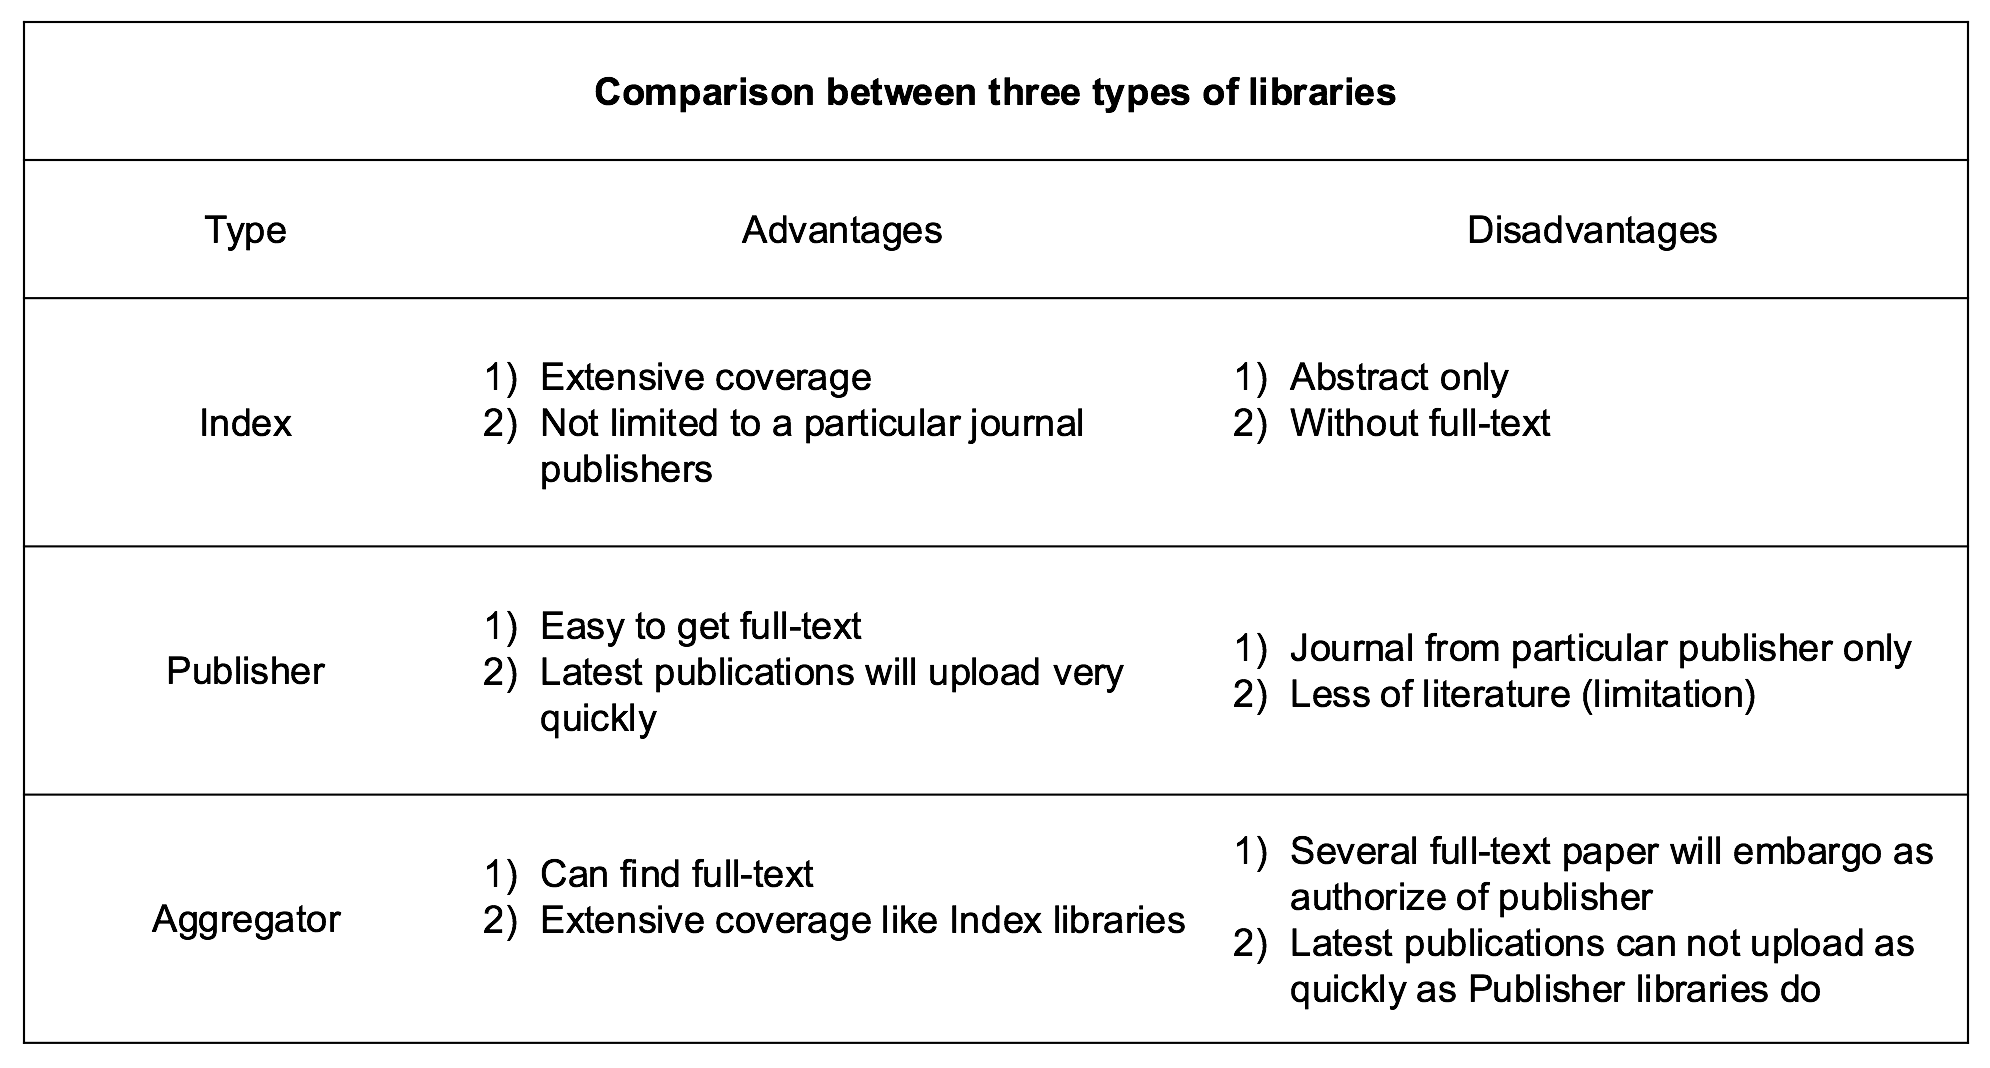
\includegraphics[width=0.8\textwidth]{Wolverine_Background_Chart_1}
	\end{center}
	\caption{Comparison between three types of libraries.\label{WBC1}}
\end{figure*}
\newpage

\subsubsection{Introduction to libraries }\todo{Consider to change the title.}

\begin{enumerate}
	
	\item\textbf{PubMed}
	\setlength{\parindent}{1em}
	 PMC (PubMed Central) is launched in 2000.
	 PubMed citations often include links to the full-text article on the publishers' Web sites or in PMC and the Bookshelf.
	 PubMed is a free library which is used for searching reference papers and abstracts related to the biomedical topics.
	 The largest subset of PubMed is MEDLINE, which is a bibliographic database containing life sciences and biomedical information.
	 Both of them are built by National Library of Medicine.You may limit your search to MEDLINE only in PubMed.
	 
	 A strong feature of PubMed is its ability to link MeSH(Medical Subject Headings) terms automatically. 
	 It is useful for people who want to find the medical articles. 
     Simple searches on PubMed can be carried out by entering tje key words of a subject into PubMed's search window.
     PubMed translates this initial search formulation and automatically adds field names.
	 Like several libraries, one can find the specific result he desires by addding relevant MeSH terms, synonyms and Boolean operators.
	 
	 The design philosophy of PubMed is based on full-text XML files, which are readable by both the machines, humans and moreover technology independent.
	 PubMed is classified into Index libraries, which is the prime reason that it is not able to provide full text in some papers.
	 For the type of database used by PubMed is Microsoft SQL server, which is a relational database to store all of 
	 the archives such as XML, images, PDF files supplementary, etc.
	  
		
	\item\textbf{IEEE Xplore}
	\setlength{\parindent}{1em}
	
	The IEEE is an acronym for Institute of Electrical and Electronics Engineers, which is one of the leading standard organizations in the world 
	It is one of the most professional organization devoted to advancing technology for the benefit of humanity.
	There are more than 420,000 IEEE members in over 160 countries.
	And IEEE Xplore is a scholarly research library formerly known as IEEE/IET Electronic Library (IEL).
	The articles covered by IEEE Xplore are mainly from the Institute of Electrical and Electronics Engineers (IEEE) and the Institution of Engineering and Technology.
	More than 3.5-million full-text documents in the field of electrical, engineering, computer science and electronics are provided in this library. 
	
	There are many features in IEEE. IEEE can rank the articles according to their click through rates or download times. 
    Once an articles is updated by the author, those who set research alert on it will receive a notification through email by IEEE.
    However, some of the features are available for members only.
    Many enterprises and schools are the members of IEEE.

	
	The front and user interface of IEEE library present the information on the screen, 
	including the latest Angular, Jquery, HTML 5, CSS.
	Most of the HTML for PDF, either it is for journal (conference) articles or standards get dynamic transformations real time and served through MarkLogic.
	Endeca, which is an Oracle product powers Xplore searches, is used in the search layer.
	All PDF files are fed through Endeca system.
	Endeca servers will provide the matching documents and Xplore platform will presents it on the screen to the user.
	And all the content is stored in oracle metadata which will be consumed by Endeca, MarkLogic Authentication, and Authorization services.
	
	\item\textbf{EBSCOhost}
	\setlength{\parindent}{1em}

	EBSCOhost is a popular reference which authorizes users to gain a great many full-text articles from proprietary databases.
	EBSCO Information Services, headquartered in Ipswich, Massachusetts, 
    which is a division of EBSCO Industries Inc., 
    the third largest private company in Birmingham, Alabama, with annual sales of nearly $2$ billion according to the BBJ's 2013 Book of Lists.

    EBSCO offers library resources to customers in academic, medical, K–12,  
    public library, law, corporate, and government markets. 
	Its products include EBSCONET, a complete e-resource management system,
    and EBSCOhost, which supplies a fee-based online research 
    service with 375 full-text databases, a collection
    of 600,000-plus ebooks, subject indexes, point-of-care 
    medical references, and an array of historical digital archives.

    In 2010, EBSCO introduced its EBSCO Discovery Service (EDS) to institutions,
    which allows searches of a portfolio of journals and magazines

	\item\textbf{Google Scholar}
	\setlength{\parindent}{1em}
	
	Google Scholar is a freely accessible web search engine that indexes the full text or metadata of scholarly literature across an array of publishing formats and disciplines. Released in beta in November 2004, the Google Scholar index includes most peer-reviewed online academic journals and books, conference papers, theses and dissertations, preprints, abstracts, technical reports, and other scholarly literature, including court opinions and patents. While Google does not publish the size of Google Scholar's database, third-party researchers estimated it to contain roughly 160 million documents as of May 2014 and an earlier statistical estimate published in PLOS ONE using a Mark and recapture method estimated approximately $80-90$ coverage of all articles published in English with an estimate of 100 million. This estimate also determined how many documents were freely available on the web.
	
	Google Scholar is similar in function to the freely available CiteSeerX and getCITED. It also resembles the subscription-based tools, Elsevier's Scopus and Thomson Reuters' Web of Science.
	
	Google Scholar allows users to search for digital or physical copies of articles, whether online or in libraries.It indexes "full-text journal articles, technical reports, preprints, theses, books, and other documents, including selected Web pages that are deemed to be 'scholarly.'" Because many of Google Scholar's search results link to commercial journal articles, most people will be able to access only an abstract and the citation details of an article, and have to pay a fee to access the entire article. The most relevant results for the searched keywords will be listed first, in order of the author's ranking, the number of references that are linked to it and their relevance to other scholarly literature, and the ranking of the publication that the journal appears in.
	
	Using its "group of" feature, it shows the available links to journal articles. In the 2005 version, this feature provided a link to both subscription-access versions of an article and to free full-text versions of articles; for most of 2006, it provided links to only the publishers' versions. Since December 2006, it has provided links to both published versions and major open access repositories, but still does not cover those posted on individual faculty web pages;[citation needed] access to such self-archived non-subscription versions is now provided by a link to Google, where one can find such open access articles.
	
	Through its "cited by" feature, Google Scholar provides access to abstracts of articles that have cited the article being viewed. It is this feature in particular that provides the citation indexing previously only found in CiteSeer, Scopus and Web of Science. Through its "Related articles" feature, Google Scholar presents a list of closely related articles, ranked primarily by how similar these articles are to the original result, but also taking into account the relevance of each paper.
	
	As of July 2013, Google Scholar is not yet available to the Google AJAX API.\\
	
	Google Scholar's legal database of US cases is extensive. Users can search and read published opinions of US state appellate and supreme court cases since 1950, US federal district, appellate, tax and bankruptcy courts since 1923 and US Supreme Court cases since 1791. Google Scholar embeds clickable citation links within the case and the How Cited tab allows lawyers to research prior case law and the subsequent citations to the court decision.The Google Scholar Legal Content Star Paginator extension inserts Westlaw and LexisNexis style page numbers in line with the text of the case.\\
	
	While most academic databases and search engines allow users to select one factor (e.g. relevance, citation counts, or publication date) to rank results, Google Scholar ranks results with a combined ranking algorithm in a "way researchers do, weighing the full text of each article, the author, the publication in which the article appears, and how often the piece has been cited in other scholarly literature". Research has shown that Google Scholar puts high weight especially on citation counts and words included in a document's title. As a consequence, the first search results are often highly cited articles.\\
		
	Limitations and criticism
	Quality — Some searchers consider Google Scholar of comparable quality and utility to commercial databases.The reviews recognize that its "cited by" feature in particular poses serious competition to Scopus and Web of Science. An early study, from 2007, limited to the biomedical field, found citation information in Google Scholar to be "sometimes inadequate, and less often updated". The coverage of Google Scholar may vary by discipline compared to other general databases.
	
	Coverage — Especially early on, some publishers did not allow Scholar to crawl their journals. Elsevier journals have been included since mid-2007, when Elsevier began to make most of its ScienceDirect content available to Google Scholar and Google's web search. As of February 2008 the absentees still included the most recent years of the American Chemical Society journals. Google Scholar does not publish a list of scientific journals crawled, and the frequency of its updates is unknown. It is therefore impossible to know how current or exhaustive searches are in Google Scholar, although a recent study estimates that Google Scholar can find almost $90$ (approximately 100 million) of all scholarly documents on the Web written in English. Nonetheless, it allows easy access to published articles without the difficulties encountered in some of the most expensive commercial databases.
	
	Matthew effect — Google Scholar puts high weight on citation counts in its ranking algorithm and therefore is being criticised for strengthening the Matthew effect; as highly cited papers appear in top positions they gain more citations while new papers hardly appear in top positions and therefore get less attention by the users of Google Scholar and hence fewer citations.
	
	Google Scholar effect – It is a phenomenon when some researchers pick and cite works appearing in the top results on Google Scholar regardless of their contribution to the citing publication because they automatically assume these works’ credibility and believe that editors, reviewers, and readers expect to see these citations.
	
	Incorrect field detection — Google Scholar has problems identifying publications on the arXiv preprint server correctly. Interpunctuation characters in titles produce wrong search results, and authors are assigned to wrong papers, which leads to erroneous additional search results. Some search results are even given without any comprehensible reason.
	
	Vulnerability to spam — Google Scholar is vulnerable to spam. Researchers from the University of California, Berkeley and Otto-von-Guericke University Magdeburg demonstrated that citation counts on Google Scholar can be manipulated and complete non-sense articles created with SCIgen were indexed from Google Scholar. They concluded that citation counts from Google Scholar should only be used with care especially when used to calculate performance metrics such as the h-index or impact factor. Google Scholar started computing an h-index in 2012 with the advent of individual Scholar pages. Several downstream packages like Harzing's Publish or Perish also use its data. The practicality of manipulating h-index calculators by spoofing Google Scholar was demonstrated in 2010 by Cyril Labbe from Joseph Fourier University, who managed to rank "Ike Antkare" ahead of Albert Einstein by means of a large set of SCIgen-produced documents citing each other (effectively an academic link farm).
	
	Inability to shepardize case law — As of 2010, Google Scholar was not able to shepardize case law, as Lexis can.
	
	Lack of screening for quality — Google Scholar strives to include as many journals as possible, including predatory journals, which "have polluted the global scientific record with pseudo-science, a record that Google Scholar dutifully and perhaps blindly includes in its central index."\\
	
	\item\textbf{Comparison Xplore}
	\setlength{\parindent}{1em}
	
	PubMed is a free library which contains many databases, like Medline, PreMedline and Publisher Supplied Citations.
    Medline is the largest subset of PubMed.
    One can also access MEDLINE through EBSCOhost.  
    EBSCOhost promises a large number of databases. 
	Many of them, such as MEDLINE and EconLit, are licensed from web content vendors.
    Others, such as Criminal Justice Abstracts, MasterFILE, are compiled by EBSCO itself.

    However, in contrast to other two libraries, the advanced search of PubMed is weak. 
    It does not show citation times or further information.
    And the only database which does not provide full-text documents is PubMed. 

    The documents in PubMed are almost related to the biomedical topics.
    IEEE contains more than one third documents in the field of electrical, engineering, computer science and electronics.
    And the articles in EBSCOhost comprises many fields, like business, education, laws, medical, computer science, and so on.

    Each library has its own features. PubMed can link the MeSH. EBSCOhost can be searched for the videos or photos concerned with the key words you enter. 
    IEEE has many features the other two databases don’t have, like “top downloads list”, “top search terms” and “custom setting” mentioned above.

    

\end{enumerate}

\todo[inline]{You need to add at least one library example of each library type, since you started with different types. Otherwise you could have focused on one type and motivated the focus. For the libraries containing articles you should add several since you are building one. You should also discuss the database techniques, including alternative ones to the used ones, such as MongoDB, Hadoop, etc. Try to compare features.}

	\section{Methods}
	\label{Methods}
	
	%%%%%%%%%%%%%%%%%%%%%%%%%%%%%%%%%%%%%%%%%%%%%%%%%%%%%%%%%%%%%%%%%%%
% Method
% Team:
% Wolverine
% Members: 
% Eric Lee, Jacky Wu, Karthick Mani, 
% Eric Chang, Dexter Chen, Peter Chen
% Relative files:
% Method_Wolverine.tex, Library.bib, WolverineChart.png
% Note:    
% Do not compile this file compile Main.tex to get the pdf file instead.
%%%%%%%%%%%%%%%%%%%%%%%%%%%%%%%%%%%%%%%%%%%%%%%%%%%%%%%%%%%%%%%%%%%

\subsection{Built a database containing ten thousand articles}

We want to build a database contains 10,000 articles.
To reach that target, we will discuss the advantages and disadvantages of different kind databases and decide the most suitable one to be the database of this study.
At a meantime, we also focus on how to use web crawlers to download articles automatically, which is contained in the database of this study.

\subsubsection{Database Management Systems}

A database is an organized collection of data, and database management systems (DBMS) are applications that can capture and analyze data.
There are many disciplines to manage data in different databases such as tables, queries, or other objects. 
The data are organized typically in a way according to the kind of database management. 

The relational database model was proposed by Edgar Codd in 1970 initially.
However, it was not universal at that time because of the lack of the technical requirements.
Until the 1980s, the first commercial relational database management system(RDBMS) which is the most popular database management system(DBMS) at present began to appear.
Besides RDBMSs, there are several kinds of DBMSs.
For example, object-oriented databases(OODBMS) and graph database management systems(GDBMS).
In accordance with the definition, a database management system (DBMS) is a computer software application that interacts with the user, other applications, and the database itself to capture and analyze data.
Well-known DBMSs include MySQL, PostgreSQL, Microsoft SQL Server, Oracle, Sybase and IBM DB2.
Furthermore,they can support different kinds of databases.




\begin{enumerate}
	
	
	\item\textbf{Object-oriented database}
	\setlength{\parindent}{1em}		
	
	An object database, which is also called object-oriented database management system(OODBMS), is a database management system restoring information in the form of objects as used in object-oriented programming.
	Object databases are different from relational databases which are table-oriented.
	Because of tighter integration with the object-oriented language, 
	the program is easier to maintain consistency with the same representation in both OODBMS and programming language.
	Although relational databases might be similar to object-oriented databases, they are actually different.
	The object-oriented database supports objects, classes, and inheritance in the database schema and query language.
	
	There are many advantages for OODBMS compared to the relational database management system (RDBMS) such as the performance, flexibility, and development cost.
	OODBMS also have some disadvantages, they have mentioned 3 disadvantages for OODBMS.
	First, the usage is forced to be similar to an object-oriented language.
	This causes difficulty when it comes to maintaining and evolving.
	Second, the technique for storing complex type of information spends many additional computational resources.
	Third, the absence of a standard data model leads to designing errors and inconsistencies.
	
	
	
	\item\textbf{Relational database}
	\setlength{\parindent}{1em}	
	A relational database is the most popular database used in the world.
	Each row in a table has its own key. 
	They can organize data into one or more tables of columns and rows, with the key identifying each row.
	Rows are also called records or tuples.
	Generally, each table represents one "entity type" (such as customer or product).
	The rows represent instances of that type of entity (such as "Lee" or "Iphone 6"), 
	and the columns representing values attributed to that instance (such as address or price).
	
	When it comes to the method for organizing the data, the relational database is easier to understand and more flexible to manipulate the data.
	Besides, SQL is simple in the relational database approach.
	For data organized in other structure, the query language either becomes complicated or extremely limited in its capabilities.
	However, once the attributes of data increases, a larger amount of tables to store your information is needed.
	Obviously, this causes the performance of relational database decreases.


	
	
	\item\textbf{Graph database}
	\setlength{\parindent}{1em}	
	A graphical database uses graph structures for semantic queries with nodes, edges, and properties to represent and store data.
	Most of them are NoSQL in nature and store data in a key-value store or a document-oriented database.
	Graph databases are powerful tools for graph-like queries, for example, computing the shortest path between two nodes in the graph.
	
	As far as we know, relational databases are the most popular databases in the world.
	In comparison, graph databases still have several advantages.
	A graph database is often faster for associative data set and map more directly to the structure of object-oriented applications.
	They can scale more naturally to large data sets as they do not typically require expensive join operations.
	As they depend less on a rigid schema, they are more suitable for managing ad hoc and changing data with an evolving schema.
	
	On the other hand, graph database also comes with some disadvantages.
	For example, the relational database is typically faster at performing the same operations on large numbers of data elements than graph databases.
	
	\item\textbf{Summary}
	\setlength{\parindent}{1em}	
	To sum up, there are several methods to store data according to the database structures.
	Two main directions are storing inside the database and storing out of the database.
	The comparison of three databases is shown in Figure \ref{WMC2}.
	
	We suggest not to store binary data in the database if it is large.
	It may cause the performance decreases significantly and the necessity of additional storage space.
	In contrast, we suggest to store binary data in the file system and record the path in the database.
	It may not cause the disadvantages above when large binary data store into the database, 
	but the binary data can not automatically distribute with the database.
	We suggest sorting the PDF file in the file system, 
	since the PDF file will cost some performance issues even though it occupies little size and our system has no requirement for automatic distribution.
	
	\begin{figure*}[ht]
		\begin{center}
			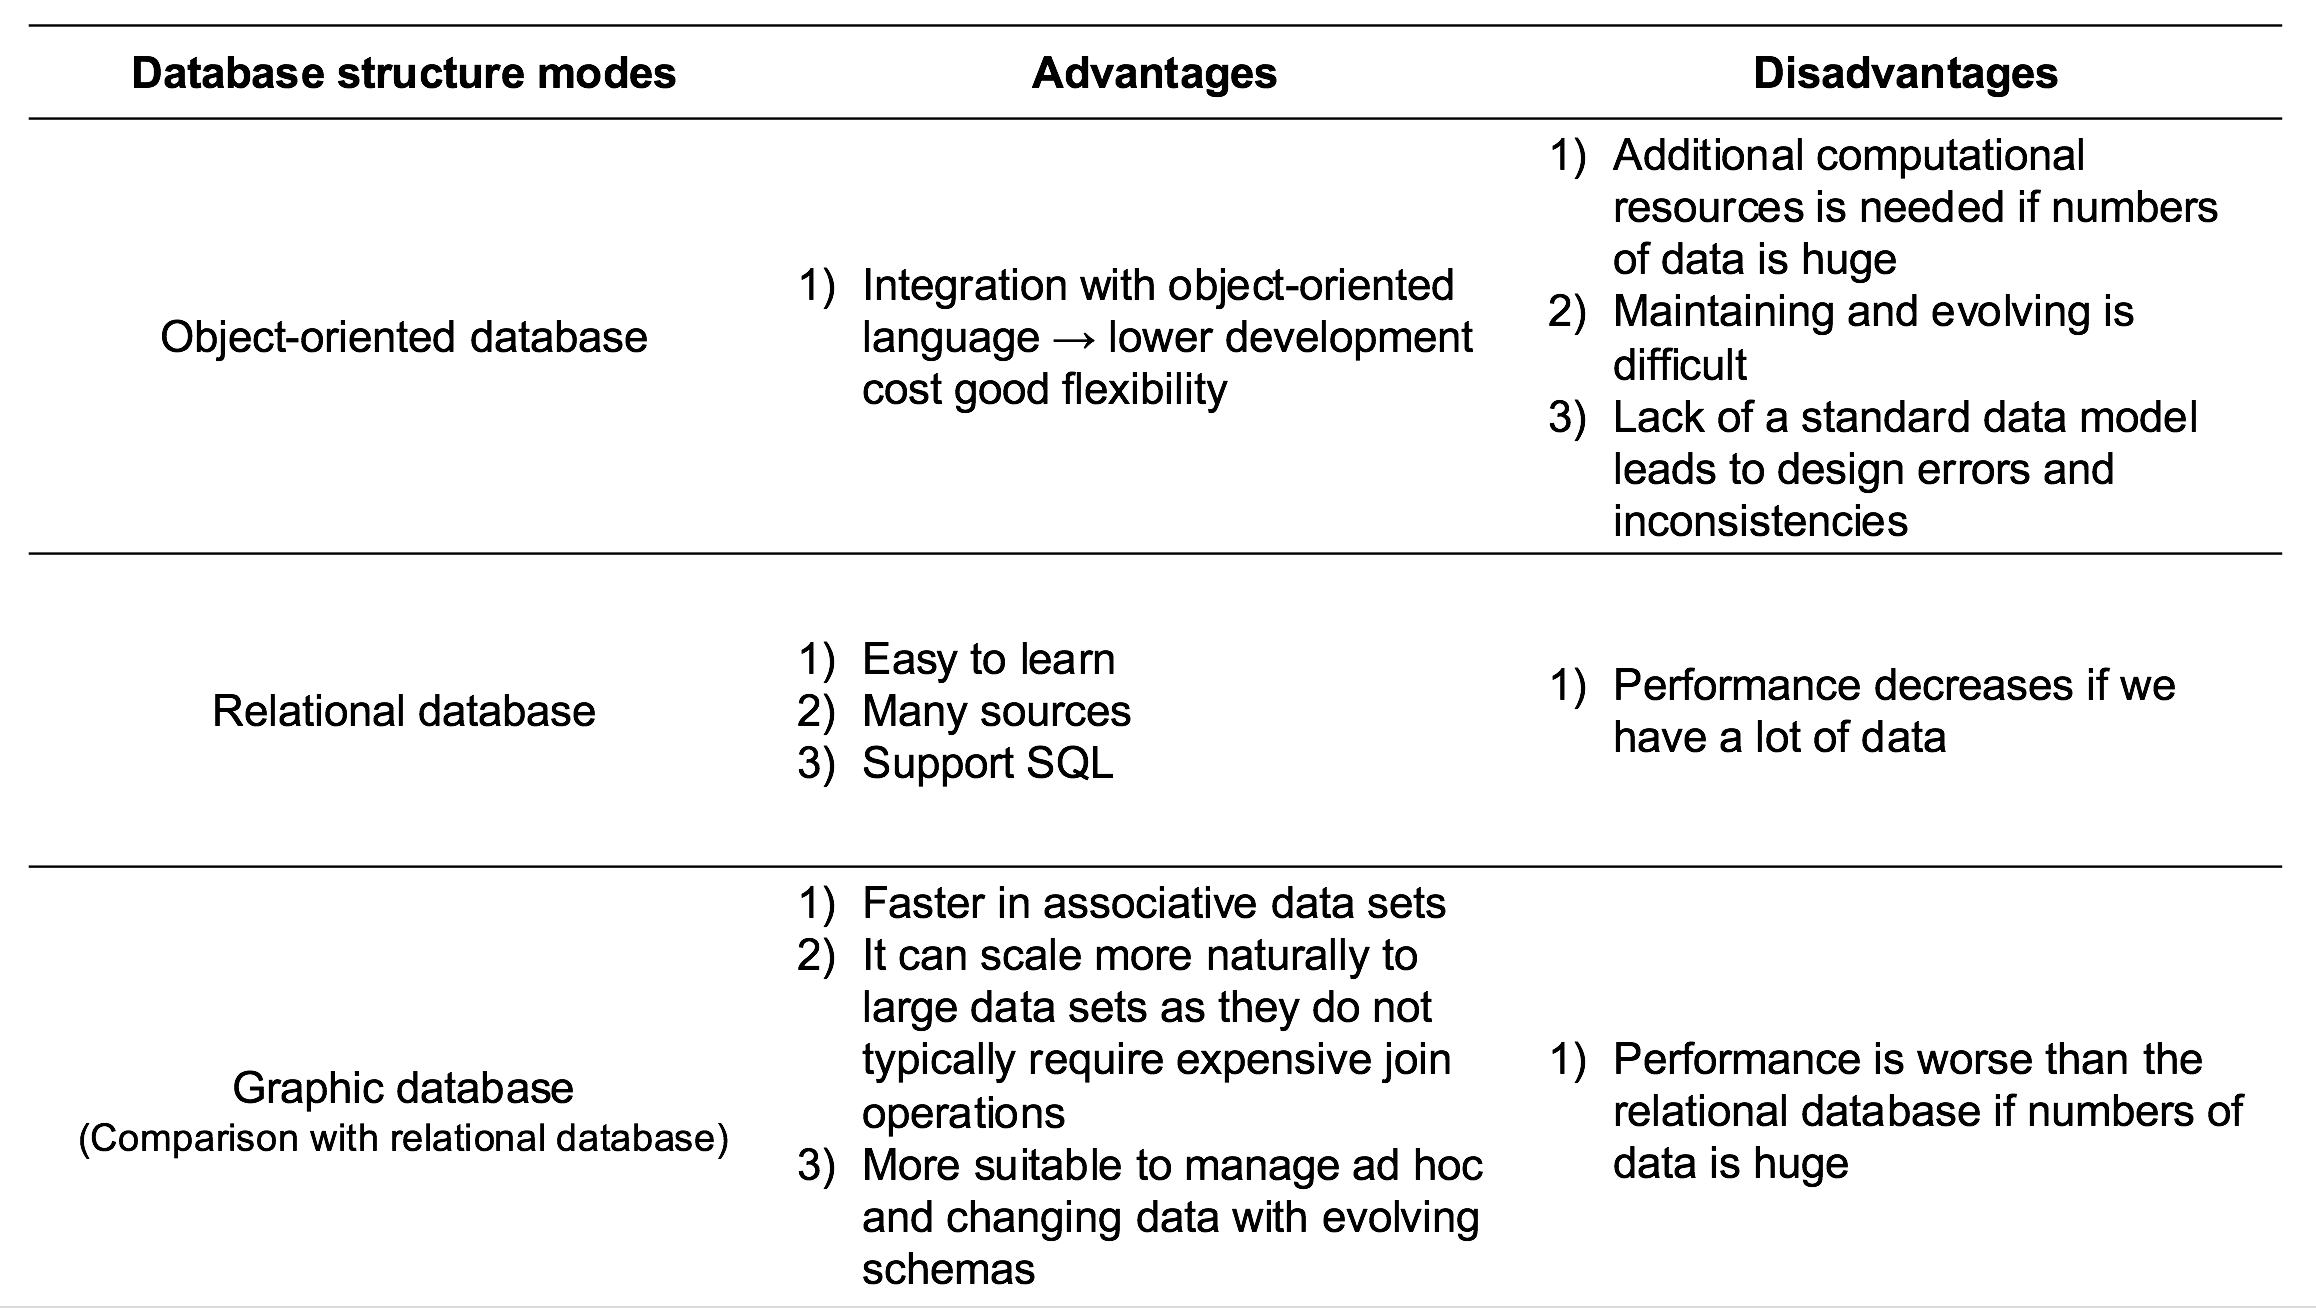
\includegraphics[width=1.8\columnwidth]{Wolverine_Method_Chart_2}
		\end{center}
		\caption{Advantages and disadvantages between three kind of databases.\label{WMC2}}	
	\end{figure*}
	
\end{enumerate}

\subsubsection{SQL and NoSQL}

Every website is full of data, such as Facebook, Bank of Taiwan and official web page of National Cheng Kung University (NCKU).
The database is coming in many forms, including Object-oriented, graph and relational, which are listed above.
Most of the databases come with querying languages interact with databases.
SQL (Structured Query Language) is the most popular among them.
It is also an American National Standards Institute (ANSI) standard.
SQL is a kind of simple language.
It is like English that helps you "communicate" with database server.
Therefore, even the people who are not good at programming can program it easily.


SQL has been a single standard to support all kinds of databases for several decades.
It seems good enough to let us don't need any alternatives.
However, it is going to be changed.
NoSQL is going to be an alternative, which means "non SQL" or "non relational".
It is different from relational database management system (RDMS) in some ways.
For example, NoSQL uses the concept of JSON-like (JavaScript Object Notation) or name-value to store data, instead of using tables like SQL.

However, both SQL and NoSQL have their own advantages and disadvantages.
Therefore, it should be chosen depending on the characteristic of data.
SQL is the ideal language when projects require logical related discrete data that can be identified and data integrity is essential.
On the other hand, NoSQL can be the ideal language if projects require unrelated, indeterminate or evolving data and simultaneously. 
It needs speed and scalability.



\subsubsection{SQLite}
SQLite is an amazing library that gets embedded inside the 
application that makes use of. It also offers an amazing 
set of tools to handle all sorts of data with much less 
constraint and ease. The following data types are supported 
by SQLite: NULL, INTEGER, REAL, TEXT, BLOB. SQLite is file
based which makes it extreme portable and can offer more than 
what is needed for development with the simplicity of working 
with a single file and a linked C based library. Thus, it's 
great for developing and even testing.

\subsubsection{MySQL}
MySQL is the most popular one among the large-scale database servers due to its rich feature and open-source product which powers lots of web-sites and applications online. 
The following data types are supported by MySQL: INTEGER, FLOAT, DOUBLE, DECIMAL, DATE, TIME, CHAR, BLOB, TEXT, ENUM. MySQL is scalable powerful which can handle a lot of data. 
Besides, it has a free community. 
Due to the cross platform, MySQL is a good choice for both development process which works on almost all platforms and for companies with heterogeneous IT infrastructure.
For developers, MYSQL is well known for its efficient workbench tool, admin and data migration which is fast on simple queries.

\subsubsection{PostgreSQL}
PostgreSQL is an open source object-relational database management system (ORDBMS) which has the main goal of being standards-compliant and extensible. 
The following data types are supported by PostgreSQL: boolean, bytea, character, date, double, integer, text, time [(p)], tsquery, xml, and so on. 
Here are the advantages of PostgreSQL.
\begin{enumerate}
	\item It's an open-source SQL and standatd compliant RDBMS. 
	\item It is also adorned with many great and open-source third-party tools for designing, managing and using the management system.
	\item Besides, it has a strong community through which a large amount of knowledge-transfer happens between experienced professional to the amateur developer.
\end{enumerate} 
 

\subsubsection{MongoDB}
MongoDB is an open-source document-oriented database. 
In this case, documents are created and stored in Binary JSON (JavaScript Object Notation) format which enables transferring data between servers and web apps with the use of the human-readable format. 
Besides, MongoDB can store the file as a file system, called Grid file system, 
storing a file into several parts separately, instead of a single document. 
That is why MongoDB can create a load-balance and fault-tolerant system effectively. 
Moreover, the use of dynamic schemas make MongoDB eliminates the need to pre-define the structure. 
Such model allows hierarchical relationships representation, array storage, and ability to change the records structure by simply adding or deleting fields.


\subsubsection{Comparison between four databases}
In comparison with PostgreSQL, there is generally no good reason to use MySQL. 
However there are certain advantages as show in can be found on Figure \ref{CompareDatabase}. which made us to choose PostgreSQL as our database in our project.
PostgreSQL is a relational database. 
It specialists in tracking the relationship between pieces of data and helping you retrieve something if you know something related to it.

\begin{figure*}[htb]
	\begin{center}
		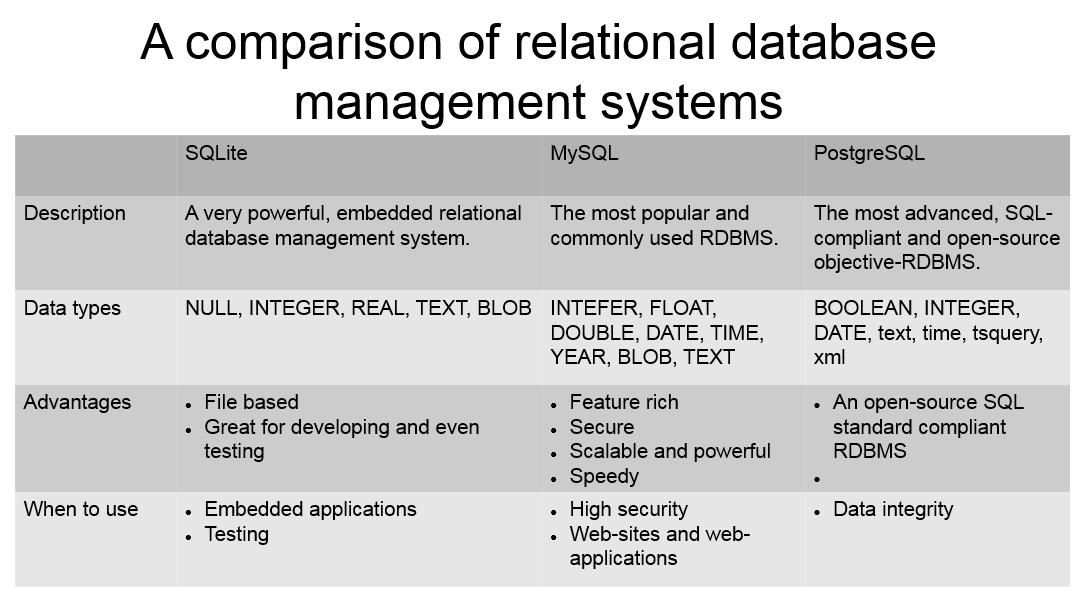
\includegraphics[width=0.8\textwidth]{CompareDatabase}
	\end{center}
	\caption{Comparison between three types of database.\label{CompareDatabase}}
\end{figure*}
\newpage

All SQL databases can do relational queries like this, but PostgreSQL is better at doing this. 
Besides, it also support the data type of "tsquery." which means it can perform full text search.


MongoDB is not a graph database, or even a relational database. 
Like CouchDB, it's a document database and it represents the other end of the scale. 

\subsubsection{Web Crawler}

	
	The web crawler is a program that can automatically browse through web pages, find out the information we assigned and store them.
	It has ability to process the data quickly and accurate to update a very large amount of data which are constantly being updated according to \cite{Liu2012}.
	It starts with a list of URL to visit, called the seeds.
	As crawler visits these URL, it identifies all the informations that we want, such as hyper links in the page and adds them to the list of URL to visit, called the crawl frontier.
	URL from the frontier is recursively visited according to a set of policies.
	If the crawler is performing archiving of websites, it copies and saves the information as it goes.
	The archives are usually stored in such a way they can be viewed, read and navigated as they were on the live web, but are preserved as 'snapshots' from \cite{Du2013}.
	We need to build up a web crawler to automatically visit a list of web page.
	Then find out which link in the page is valuable to download into our database.
	
	

\newpage % Ends the current page and causes all figures and tables to be printed

	%%%%%%%%%%%%%%%%%%%%%%%%%%%%%%%%%%%%%%%%%%%%%%%%%%%%%%%%%%%%%%%%%%%%%%%%%%%%%%%%%%%
% Team:
% EagleUnit
% Members: 
% Chinweze Ubadigha, Feng-Chun Hsia, Henry Peng, I-Chieh Lin, Jones Hou, Piyarul Hoque, Ray Chang
% Relative files:
% Main.tex, Background_EagleUnit.tex, Library.bib, EagleUnit_Background_Chart_1.png
% Note:
% Do not compile this file compile Main.tex to get the pdf file instead.
%%%%%%%%%%%%%%%%%%%%%%%%%%%%%%%%%%%%%%%%%%%%%%%%%%%%%%%%%%%%%%%%%%%%%%%%%%%%%%%%%%%
\subsection{Webpage Construction}
\textit{\footnote size Author : Chinweze Ubadigha, Feng-Chun Hsia, Henry Peng, I-Chieh Lin, Jones Hou, Piyarul Hoque, Ray Chang.}\\

We are going to construct a public, user friendly web site, which provide service of scientific article searching.
To achieve this goal, we separate our responsibility into parts:\\
\begin{itemize}
	\item Build up the web server.
	The web server is basically built using Django web frame work on a CentOS 7 system. Django is a web framework which is constructed using Python code.
	For the purpose of this project the Django web server was built using PostgresSQL (database management application), 
	Nginx (traffic control and security), and 
	Gunicorn (interface to translate clients requests in HTTP to python calls that Django can understand)  
	and Python WSGI HTTP Server (used to create entry sock for Django)
	thus making a robust web server.
	\item Build a web page with a search bar.
	\item Place a list on the webpage which showing the search results.
	\item Build a metadata schema which contains all information in a PDF and then edit it in an XML structure. 
	\item Build up the APIs. The search bar should send the search string and the result list to tje search system 
	then the system receive the results of searching and display it.
\end{itemize}
This article will provide a review through the tools and methodologies we use to achieve each work.
\subsubsection{Web Server}
For any web page, a web server is necessary.
There are three web server system used in our project. 
They play the role as web page framework, reverse proxy server, 
and database management, respectively.
Consider the ease to use and learn, and the generality of Python language 
that we choose Django, a Python based web server system for our work.
\subsubsection{Ngnix}
Nginx is a high performance web server. It can act as an HTTP and reverse proxy server. When compared to Apache, Nginx is light-weight and has minimal hardware requirements to deal with web traffic. It has many features as follow:
\begin{itemize}
	\item Fastest and the best for serving static files
	\item Increased security of server 
	\item Handling many concurrent connections at the same time
	\item Load Balancing Support
\end{itemize}
\subsubsection{Django}
Django is one of the most well-known python web framework. There are many famous sites built with Django, such as Pinterest, Instagram, Disqus. It has many features as follow:
\begin{itemize}
	\item Free and open-source web framework
	\item Written in python
	\item MTV framework
	\item fast and secure
	\item Exceedingly scalable
	\item Fully loaded
	\item Incredibly versatile
\end{itemize}
Next, we are going to show how to install Django in Linux.
\begin{itemize}
	  
		\item Step 1\\
		Open the terminal and create folder named mydjango
			\begin{itemize}
				\item\emph {\$ mkdir mydjango}\\
				\item\emph {\$ cd mydjango}
			\end{itemize}	
		\item Step 2\\
		Create a vitual environment named mydjangovenv
			\begin{itemize}
				\item\emph {/mydjango \$ virtualenv mydjangovenv}\\
				\item\emph {/mydjango \$ cd mydjangovenv}\\
				\item\emph {/mydjangovenv \$ source bin/activate}
			\end{itemize}	
		\item Step 3\\
		Install django
			\begin{itemize}
				\item\emph {(mydjangovenv) \$ python -m pip install django}\\
			\end{itemize}	

After installing Django, we can start to build websites. Fisrt we need to create project and apps. One project can contains many apps. In pratical, these apps are divided into different funtions and can be reused. 
		\item Step 4\\
		Create a project named mysite and make it run in server
			\begin{itemize}
				\item\emph {(mydjangovenv) \$ django-admin.py startproject mysite}\\
				\item\emph {(mydjangovenv) /mysite \$ python manage.py runserver 0.0.0.0:8000}
			\end{itemize}	
		\item Step 5\\
		Create apps named firstapp
			\begin{itemize}
				\item\emph {(mydjangovenv) /mysite \$ python manage.py startapp firstapp}\\
			\end{itemize}

Then, we will introduce some key files for designing a webpage.
		
		\item \textbf{views.py}\\
			  In the views file, it contain many funtions to deal with HttpRequest and  HttpResponse objects.
		\item \textbf{urls.py}\\
			  This file defines URL configuration, which is the relationship between the view funtions and the URL.
		\item \textbf{templates}\\
			  Templates is file which consist of some HTML/CSS desiged webpage. Therefore, the view funtions can call these webpage for a request.
		\item \textbf{model.py}\\
			  Nowadays, webpages usally interact with users, in order to store the information input by users, we need to connect with database. The model file define the schema of database and make it easy to synchronize information.\\\\
With the basic knowledge above, we can start to build a funtional and compelete website in Django.
\end{itemize}
\subsubsection{Django with Postgres, Nginx, and Gunicorn}

	%%%%%%%%%%%%%%%%%%%%%%%%%%%%%%%%%%%%%%%%%%%%%%%%%%%%%%%%%%%%%%%%%%%%%%%%%%%%%%%%%%%
% Team: Rainy
% Members: Rain  Dickson  Sareddy
% Relative files:
% Note: Do not compile this file compile Main.tex to get the pdf file instead.
%%%%%%%%%%%%%%%%%%%%%%%%%%%%%%%%%%%%%%%%%%%%%%%%%%%%%%%%%%%%%%%%%%%%%%%%%%%%%%%%%%%
\subsection{Latent Semantic Analysis}
Latent Semantic Analysis is a kind of Corpus-Based similarity anaysis. Corpus-Based similarity is a semantic similarity measure which determines the similarity between the words based on the information gained from corpora. A Corpus is a large collection of texts and it is used for language research. Latent Semantic Analysis(LSA) assumesthat the words with close meaning will mostly occur inthe similar group. A matrix which contains word counts per paragraph was constructed from a  dataset.In order to reduce the number of columns, singular ue decomposition (SVD) is used and it preserves the similarity structure among the rows. The LSA approach is extended by focusing on term vectors instead of the representation of dual document-term and cosine measures between the vectors are expressed based on the semantic relatedness between two texts.
 
\subsection{Metadata Extraction}
Metadata Extractor is the module which can extract metadata in PDF files such as title, subheading, doi, etc. We use python package pyPdf to extract metadata directly and use metadata to do a couple of things. First, we extract titles of articles returning those to the web page as search results. Second, we use metadata extractor to extract subheadings which are treated as the definition of break point to split PDF file i.e. one article will be separated into small pieces based on subheading. The small pieces will convert into .txt files by the .txt converter we built so that we can take .txt files into similarity comparison and get the most relative parts in the article. Third, we extract doi from the article. 

 \subsection{Text Processing}
 After converting an article from .pdf file format to .txt format, we read the converted text file to the program and do preprocessing task. First, delete all stopwords(ex. is am are the etc) that are irrelavent to the article. Second, remove all punctuation and any non-alphabet characters  in the article. Third, tokenize the article into words and count the frequency of each word appeared in the article. Finally, remove the word only appeared once in the article because low ocurrance indicates less importance of the word to the article.

\subsection{Similarity Comparison}
	\begin{figure*}[htb]
		\begin{center}
			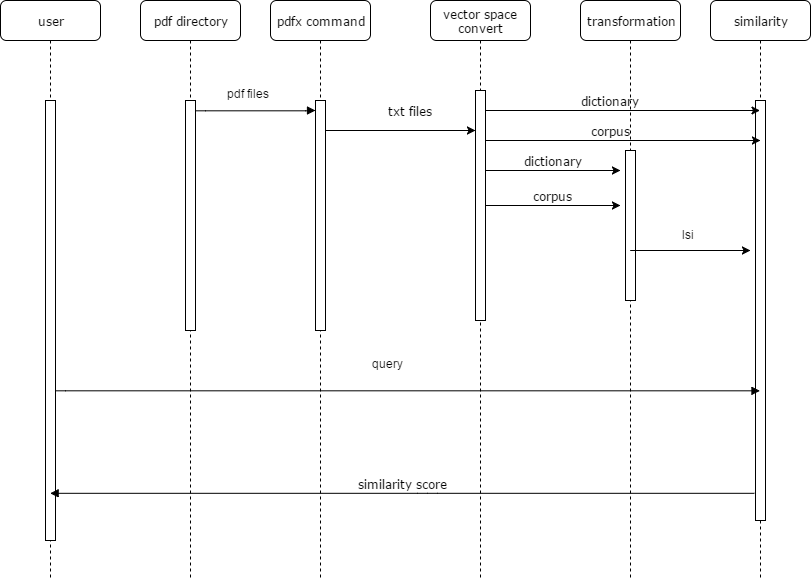
\includegraphics[width=0.8\textwidth]{Rainy_Sequence_diagram}
		\end{center}
		\caption{Sequence diagram of text similarity compare functionality.\label{Sequence diagram}}
	\end{figure*}
	\newpage
	%%%%%%%%%%%%%%%%%%%%%%%%%%%%%%%%%%%%%%%%%%%%%%%%%%%%%%%%%%%%%%%%%%%%
% Method
% Team:
% Union
% Members: 
% Bernie Huang, Jim Lan, Hoang Tan, Kenny Hsu, Rahul Aditya, Tan Phat, Wei
% Relative files:
% Method_Union.tex
% Note:    
% Do not compile this file compile Main.tex to get the pdf file instead.
%%%%%%%%%%%%%%%%%%%%%%%%%%%%%%%%%%%%%%%%%%%%%%%%%%%%%%%%%%%%%%%%%%%
\subsection{Method} %Please change "Method" to your goal. 
\textit{\footnotesize Author:Bernie Huan, Jim Lan, Hoang Tan, Kenny Hsu, Rahul Aditya, Tan Phat, Wei.}\\

As mentioned in the background, our group use natural language processing in order to generate metadata.
The scope of metatada processing is about producing at least three types of metadata including author name, title and abstract.
This is at least we want to produce within the time frame of this course.
Once accomplishing the 3 types of metadata, we will extend the scope of our project, 
intimidate the scheme to produce other remaining metadata such as doix number, journal name, volume number and so on.
If time is still on our side, we will even extend the scope of our project further and try to build a djanjo or search engine. 
Try to make our project more completely and let it can be shown on the interface. 
Following discussion are our plan to complete extracting the 4 first types of metatata from PDF files.

\subsubsection{Title extraction}

We chose python to be the program to catch the title and other metadata.
First step, we import some necessary packages and functions as following:

\begin{enumerate}
	
	\item re: Regular expression package is a useful package which could be applied to the string comparison.
	\item os: This function can connect the python to operating system, so that we can call the path of the files and folders.
	\item nltk: A natural language toolkit.	We use the corpus plaintext function to build the txt file in a folder as corpus.
	\item string:The string package includes a lot of classes such as lowercase, uppercase,punctuation,digits or whitespace...etc.
	
\end{enumerate}  

To begin, we convert all PDF files we want to deal with into a txt file,
set the path and store them in specific folder. 
Then, regular expression in python can help capturing the first sentence in the txt files, which have been converted and
stored in specific folder in previous step.
The process of extracting title from the text is mainly regulated by Union_extract_title.py. 
The coding scheme has following steps: Importation of necessary components, setting the path, creating the directory we 
will write the .txt files to after stripping text, using basic command to extract titles. 
The results are tested and listed.
We successfully produce the title of the article in a txt file.

\subsubsection{Author extraction}

In this part, we use the existing python packages to achieve our goal.
The key point in this part is natural language processing, which we have introduced in the basic section.
Also we combine the key word comparison technique to finish this task.
The following step is below:

\begin{enumerate}
	
	\item Section Separation: As we separate the abstract part from the full text, we extract the text above the 
	abstract section and rename as top section. 
	This section contains title, author and email ,etc.
	\item Tokenization: After accessing the top section, we separate the text into each single word. 
	These single words composed with a string list. 
	\item Part Of Speech Tag: We use the existing corpus to tag the part of speech to the words. 
	This step is necessary since that the chunker needs the every word's part-of-speech and then chunck.
	\item Chunker: In this part, we mainly chunk the noun because a noun often represents some meaningful features 
	such as location or author.
	\item Label: We check every phrase with the corpus which contain specific words like people name. 
	Then we label the words and store within the new list. 
	Eventually, we write the information within the xml file. 
	
\end{enumerate}

The above steps is also available to extracting the location and organization,etc when needed. 
The file mainly functioning for this task is Extract_Authors.py.
The coding scheme for this task is quite similar to title extraction.
The main different is a corpus is introduced.
This scheme also include a natural language toolkit in order to extract people's name. 
As we test the result, our program has been able to extract authors' name.

\subsubsection{Abstract extraction}

	Developing from previous theory mentioned in the background section, we use the python to catch the abstract.
	The following step is below.
	%\begin{center}
	%	\includegraphics[width=\columnwidth]{Union_Background_Chart_2
	%\end{center}
	The pdf is converted into txt file.
	Thus, it will create the txt file.
	The work is done by hand coding.
	For detailed coding scheme, we have presented it in the appendix at the end of this report.
	
	After being able to read the txt file on every line, the python will detect the content of the abstract.
	In order to do so, we strip the text between "abstract" label and "introduction" label.	
	
	
	Abstract-database:including the condition
	
	\begin{enumerate}
		
		\item Capital         "ABSTRACT".
		\item Lower case      "abstract".
		\item In the sentence "Abstract—Word sense ...".
		\item And so on...
		
	\end{enumerate}
	
	In the process building "abstract database", we are aware of different papers may have different form of structures 
	and writing style, we search through numbers of articles from different journals.
	Number of article found is 100, from 20 different journals including The Lancet, Progress in Energy and Combustion Science, Chemical Analysis and so.
	Search results for sections such as Theoretical, Methods, Results, Discussion, Conclusion, Acknowledgments are also obtained.
	Table below are the results of the search.
	
	%\begin{center}
		%\includegraphics[width=\columnwidth]{Table for method Union}.\\
		%\includegraphics[width=\columnwidth]{Table 2 for method Union}.\\
		%\caption{Result of finding all forms of "abstract", "introduction" written by different authors}
	%\end{center}
	
	Then our program will read the txt file on every line.
	If the python detects the abstract-database-stop's words ,it will stop to catch the sentences.
	abstract-database-stop:including the following conditions
	
	\begin{enumerate}
			
		\item The blank line.
		\item Specific words in the beginning "Keywords".
		\item And so on.
					
	\end{enumerate}
	
	The intended output are sentences extracted to the txt file.
	To further validate if the program can run precisely, members randomly search for articles (10 articles) to test the programs.
	The program was run successfully and all abstracts was extracted from the text.
	 	
\subsubsection{References URL extraction}

References URL extraction is very easy and straightforward.
Just use a powerful package called PDfx to complete this task.
Find the package online and use it.
The procedures are below:

\begin{enumerate}
	
	\item First of all, a PDFx package is imported to python.
	\item Second, The function in PDFx package is utilized to get the metadata and the URL of references by inputting a URL of a PDF or PDF's file name.
	\item Finally, output and list the results in txt file and choose the specific directory to store it.

\end{enumerate}
 
This method can also detects URL,arxiv and doi references.  
Plus,by using this method, we also can easily extract the title, page number and creation date. 
However,only the page number is always right in every case. 
The others are not totally correct. 
Basically, over 50 percent is not correct.
Thus, among these metadata,this method is more suitable for page number. 

\subsubsection{Search sentences}

The search sentence part is related to the search engine.
 After extracting the necessary information, we have to find a way to search these data.
 The procefure is following:
\begin{itemize}
	
	%\begin{center}
	%	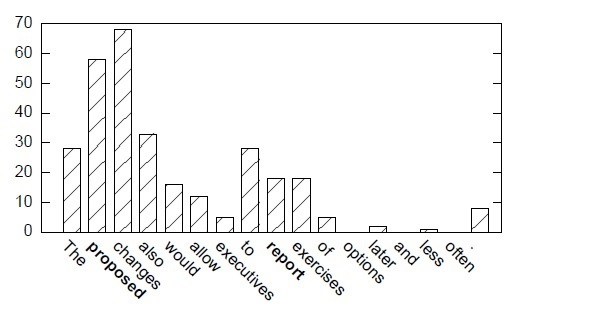
\includegraphics[width=0.8\columnwidth]{Union_Background_Chart_2}
	%\end{center}
	\item First, The PDF is converted to the txt file.(Make the program to read the file name much easier)
	\item Second, read the txt files by lines.
	\item Third, the array is created to divide the section of the articles.
	\item Fourth, The array is expanded to divide the section clearly.
	\item Fifth, Users search the sentences, the program search all the sections by this sentence.
	\item Sixth, show the results.
	
\end{itemize}
\subsection{API}
We also attempt to produce an semi-automatic interface that help users to inquire certain information from our database. 
Currently it allows user to search for abstracts, introduction, method, result, discussion, and reference. We will continue develop the interface in the remaining week. 
The objectives are either covering more functions or make the results pages has more professional appearance. However, that
said when we still have enough time.

\newpage % Ends the current page and causes all figures and tables to be printed
	
	\section{Results and discussion}
	\label{Results and discussion}
    %%%%%%%%%%%%%%%%%%%%%%%%%%%%%%%%%%%%%%%%%%%%%%%%%%%%%%%%%%%%%%%%%%%%%%%%%%%%%%%%%%%%
% Team:
% EagleUnit
% Members: 
% Chinweze Ubadigha, Feng-Chun Hsia, Henry Peng, I-Chieh Lin, Jones Hou, Piyarul Hoque, Ray Chang
% Relative files:
% Main.tex, Background_EagleUnit.tex, Library.bib, EagleUnit_Background_Chart_1.png
% Note:
% Do not compile this file compile Main.tex to get the pdf file instead.
%%%%%%%%%%%%%%%%%%%%%%%%%%%%%%%%%%%%%%%%%%%%%%%%%%%%%%%%%%%%%%%%%%%%%%%%%%%%%%%%%%%
\subsection{Web Server Structure}
By combining Django, PostgreSQL, NGINX, and Gunicorn, a robust web server was build.
The Django provide a very convenient web page framework to modify the outlooks and functions. 
For the database system, Postgres provide a much more powerful function and management then the default SQLite in Django.
By using Gunicor as an interface to the Django, NGINX makes the server more  fast and secured on communication with the internet requests.

\subsection{NGINX Server}
The NGINX server provide a particular internet domain to our web page,
which allowed us to connect the web page by using URL,
with out entering any port number. Additionally,
the NGINX server is not only playing the role of reverse proxy server of our Django server,
it can direct the user to any other domain in the main sever as well.
It means we can have other single HTML files not including in the Django server, or,
even an other Django project, and all linking to the same NGINX server.
NGINX can lead the user to projects according their own requests. 

\subsection{Web Page}
The final design of the search setting page has a search bar and several filters.
It allows users to enter the keywords, and decide which part of articles should the search system search in.
To display the articles found, we didn't shows them in the same page with search settings in the end. 
Instead, a link to a new page displaying all the metadata of search results was created.

    %%%%%%%%%%%%%%%%%%%%%%%%%%%%%%%%%%%%%%%%%%%%%%%%%%%%%%%%%%%%%%%%%%%%
% Result
% Team:
% Union
% Members: 
% Bernie Huang, Jim Lan, Hoang Tan, Kenny Hsu, Rahul Aditya, Tan Phat, Wei
% Relative files:
% Result_Union.tex
% Note:    
% Do not compile this file compile Main.tex to get the pdf file instead.
%%%%%%%%%%%%%%%%%%%%%%%%%%%%%%%%%%%%%%%%%%%%%%%%%%%%%%%%%%%%%%%%%%%

\section{Final Outcome}
\textit{\footnotesize Author:Bernie Huan, Jim Lan, Hoang Tan, Kenny Hsu, Rahul Aditya, Tan Phat, Wei.}\\
\begin{enumerate}
	\item Readable PDF on convenient software.
	\item User friendly format for searching.
	\item Free database contains 10k full text.
	\item The most important sentences can be viewed.
	\item It’s more convenient for readers by categorizing articles by fields.
\end{enumerate}
\section{Work Break Structure(WBS)}
\subsection*{Level 1}
Website for search, read online and download.
\subsection*{Level 2}
\begin{enumerate}
	\item Database for 10k articles(PDF).
	\item Xml file with necessary  information.
	\item PDF which could show in Utopia.
	\item PDF which could show in Utopia.
\end{enumerate}	
\subsection*{Level 3}	
\subsubsection*{Database}
\begin{enumerate}
	\item Web crawler.
	\item Sever.
	\item Management system.
\end{enumerate}	
\subsubsection*{Xml information}
\begin{enumerate}
	\item Journal name.
	\item Title.
	\item Authors. 
	\item Abstraction.
	\item References URL.
	\item Issue of publication.
	\item Page number.
	\item Place of publication.
	\item ISBN.
	\item Doi.
	\item Date of publication.
\end{enumerate}	
\subsubsection*{Xml information}
\begin{enumerate}
	\item List of data.
	\item Search engine.
	\item API. 
	\item User account.
\end{enumerate}	

%\begin{center}
%	\includegraphics[width=\columnwidth]{Union_Background_Chart_2
%\end{center}

%\begin{center}
  %\includegraphics[width=\columnwidth]{Table for method Union}.\\
  %\includegraphics[width=\columnwidth]{Table 2 for method Union}.\\
  %\caption{Result of finding all forms of "abstract", "introduction" written by different authors}
%\end{center}

\section*{Describe process}

\section*{Result and Discussion}


\section*{Working Plan}
%\begin{center}
%\includegraphics[width=\columnwidth]{Table for method Union}.\\
%\includegraphics[width=\columnwidth]{Table 2 for method Union}.\\
%\caption{Result of finding all forms of "abstract", "introduction" written by different authors}
%\end{center}
\section*{Conclusion}

\section*{Suggection}

	\section{Conclusions and future work}
	\label{Conclusions and future work}
    \subsection{Search Settings}

So far our search system can only provide "single query" searching, which means the users can only search with a single keyword every time.
If multiple words was entered in the search bar, it will be processed as a single word.

Nowadays, almost every existing scientific article database provides multi-query and Boolean searching function,
to make it more convenient for the user to enter all possible key words,
and faster to convert the result.
To provide a more efficient information retrieve service,
multi-query search seems to be a necessary function.

\subsection{Search Result}
Providing more detail, generating the bibliography, and refine the search result are all common functions in existing scientific article searching services.
In our system, the result pages will display the title of all articles found and the percentage of similarity number compared with search query.
Moreover, there's a visualized figure which can plot chart diagram whose x-axis is range of similarity percentage and y-axis is how many articles in those range.
However, there's no function to operate or further limit the range of searching within the result.
For next step,
building up bibliography generating function and original publisher linking will be a good direction for improvement.


    %%%%%%%%%%%%%%%%%%%%%%%%%%%%%%%%%%%%%%%%%%%%%%%%%%%%%%%%%%%%%%%%%%%
% Future Work
% Year:
% 2017
% Team:
% RCPL
% Members: 
% Lewis Hsu, Paul Lin, Tam-Van Ngo
%Team:
%Rainy
%Dickson, Rain, Sareddy
% Relative files:
% Future_work.tex
% Note:    
% Do not compile this file compile Main.tex to get the pdf file instead.
%%%%%%%%%%%%%%%%%%%%%%%%%%%%%%%%%%%%%%%%%%%%%%%%%%%%%%%%%%%%%%%%%%%

\subsection{Future Work}
So far, our web page has implemented the full-text search function. 
After clicking the search icon, it can perform the full-text search through the PDF files in the database and extracts of the most similar parts in decreasing order. 
Besides, it can also display the title and its relevance in descending order on the result web page.

However, we did not perform the search function through a PDF reader.
Instead, we provide a search box on a web page which the user cannot click on a highlighted text and thereby perform a full-text search through the PDF reader. 
Therefore, it would be great to build or find a PDF reader which the strings inside the text can be clicked and perform full-text search through the PDF files in the database as the next step of the future work.
 
The current search process took quite a bit of time to a very small size of testing samples(89 articles), the response time of the system would be much more slower when the size of database increases. 
Therefore, optimization of a database, search function and the web server is needed. 
This will enhance the user experience while searching.
 
We also hope that more searching methods can be considered and implemented to the system. 
Apart from the performance of the web service, it is also worth providing a hyperlink to the original source of PDF file and using Harvard citation format.
Last but not least, visualization of the result is needed. The website should provide charts about the distribution of similarity score of different parts of the article to the search query, also provide service to show the wanted result by selecting the relevant boxes(ex. rank by publishing year, show result based on different types of articles etc).
    

	\appendix
	\section{XML metadata sturcture}
	\label{XML}
	%%%%%%%%%%%%%%%%%%%%%%%%%%%%%%%%%%%%%%%%%%%%%%%%%%%%%%%%%%%%%%%%%%%%%%%%%%%%%%%%%%%
% Team:
% EagleUnit
% Members: 
% Chinweze Ubadigha, Feng-Chun Hsia, Henry Peng, I-Chieh Lin, Jones Hou, Piyarul Hoque, Ray Chang
% Relative files:
% Main.tex, Background_EagleUnit.tex, Library.bib, EagleUnit_Background_Chart_1.png
% Note:
% Do not compile this file compile Main.tex to get the pdf file instead.
%%%%%%%%%%%%%%%%%%%%%%%%%%%%%%%%%%%%%%%%%%%%%%%%%%%%%%%%%%%%%%%%%%%%%%%%%%%%%%%%%%%
\subsection{XML metadata structure}


To make the database functional for the user to receive the articles that they are looking for,
our responsibility will be creating an interface between the user, the database, and the searching program. 
In other words, we're going to construct a webpage with a search bar for the user to enter their search string,
and can display the search results given by the search system. 
To display the information of each article the system found, we need to construct an XML schema which contains all important data about the article.

This article provides an overview of metadata standards which are related to our responsibility.
A number of metadata schemas in use to now-a-days are reviewed, including MODS, METS, METS+MODS+PREMIS, MARC 21, MARCXML, Dublin Core, and  their pros and cons. 
Finally, we compare these schemas by examining the characteristics and unique features of them. 
We are able to rank them and suggest the optimum standard to build our XML structures. 
XML is a markup language that defines a set of rules for encoding the documents in a format,  which is both human-readable and machine-readable. 
It is widely used to representation of arbitrary data structures, such as those used in web services.

Metadata is defined as the "data about data" or alternatively "information about information." 
In practice, metadata summarizes basic information of data for the organization and management of documents. 
It can be accessed manually or by automatic information processing and coding. \cite{underwood2003xml}.

The metadata schemas can be classified into three types \cite{dempsey1997specification}:
\begin{itemize}
	\item Simple formats: It includes relatively unstructured data, typically automatically extracted from resources and indexed for searching. 
	The data has little explicit semantics and does not support searching by field, such as Lycos, Altavista, Yahoo, etc.
	\item Structured formats: It includes data which contains the full enough description to allow a user to assess the potential utility or interest of a resource without having to retrieve it or connect to it. 
	The data is structured and supports fielded searching, such as Dublin Core, IAFA templates, RFC 1807, SOIF, LDIF.
	\item Rich formats: It includes fuller descriptive formats which may be used for location and discovery, 
	but also have a role in documenting objects or very often, collections of objects, such as ICPSR, CIMI, EAD, TEI, MARC.
\end{itemize}

XML (Extensible Markup Language) is the universal format for the encoding and exchange of structured documents and data. 
There are no predefined tags and document structures in XML. 
In other words, the XML provides structural capabilities that HTML lacks, making it easy to achieve the principles of modularity and extensibility. 
The XML schema specification defines a schema language that allows for the specification of application profiles that will increase the prospects for interoperability \cite{duval2002metadata}. 
Our work is to build a metadata schema in XML structure. The following sections will introduce the schemas mentioned previously.

%%%%%%%%%%%%%%%%%%%%%%%%%%%%%%%%%%%%%%%%%%%%%%%%%%%%%%%%%%%%%%%%%%%%%%%%%%%%%%%%%%%
% 1. Different standards of metadata
%%%%%%%%%%%%%%%%%%%%%%%%%%%%%%%%%%%%%%%%%%%%%%%%%%%%%%%%%%%%%%%%%%%%%%%%%%%%%%%%%%%

\subsubsection*{Different standards of metadata}
\label{sec:mets}
There are various types of standards that describe the metadata in different fields and applications. 
Listed in the following are five different standards with brief introduction.

\begin{figure*}		
	\begin{center}
		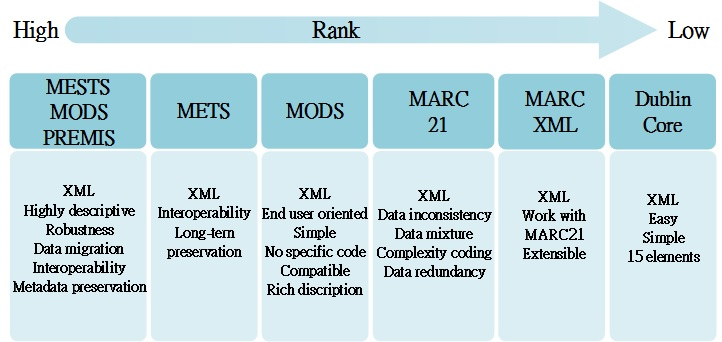
\includegraphics[width=1.8\columnwidth]{EagleUnit_Background_Chart_1}
	\end{center}
	\caption{Overview and hierarchical ranking of metadata standards and their individual features}
\end{figure*}

\begin{enumerate}
	\item METS\\
	{\bf Introduction}\\
	Metadata Encoding and Transmission Standard (METS) is an XML encoding format for storing the descriptive, administrative, structural and behavioral metadata needed to manage complex digital objects in an open and standardized way.
	
	In 1990s, Making of America II (MOA2) project was proposed to share vision between national digital libraries 
	which provides a mean for the Digital Library Federation (DLF) to investigate, refine, recommend metadata elements and encodings used to discover, display, and navigate digital archival objects.
	MOA2 DTD was created to test MOA2 project.
	
	However, MOA2 DTD was limited in several ways. 
	It provided no flexibility in terms of the exact metadata elements to be used for descriptive, administrative and structural metadata. 
	Also, limited in scope to support for text and still image materials and no attempt to support time-based media such as audio or video materials. 
	In order to solve those problems led to the creation of METS.
	
	{\bf Advantages}
	\begin{enumerate}
		\item METS to facilitate the exchange and interoperability of digital library objects across digital library systems.
		\item Provide and support a practical and flexible packaging mechanism for the long-term preservation of digital library objects.
		\item The METS standard can be considered as one of the many efforts to try to determine, for one particular community, how complex sets of data and metadata might best be encoded to support both information exchange and information longevity.
	\end{enumerate}	
	{\bf Disadvantages}
	\begin{enumerate}
		\item METS has gone some distance towards achieving these design goals, it is not itself in a guarantee of interoperability.
		\item There are some obvious practical difficulties in using METS for the long-term preservation of digital objects.
	\end{enumerate}
		

	
	%%%%%%%%%%%%%%%%%%%%%%%%%%%%%%%%%%%%%%%%%%%%%%%%%%%%%%%%%%%%%%%%%%%%%%%%%%%%%%%%%%%
	\item MODS\\
	{\bf Introduction}\\
	Metadata Object Description Schema (MODS) was developed by the Library of Congress' Network Development and MARC Standards Office in 2002. 
	It is the bibliographic element set for multiple purposes, which was especially for library applications. 
	As an XML schema, it is not only able to carry the selected data from existing MARC 21 records but to enable the creation of original resource description records. 
	It includes a subset of MARC and uses language-based tags rather than numeric ones. In some cases regrouping elements are from the MARC 21 bibliographic format. 
	It released the third version (version 3.6) in May 2015. MODS is expressed using the XML of the World Wide Web Consortium. 
	The standard is maintained by the MODS Editorial Committee with support from the Network Development and MARC Standards Office of the Library of Congress.\\
	
	MODS is an XML schema which is guidelines a resource description for encoding, as well as exchange and management descriptions of encoding.\\
	
	Elements of MODS generally inherit the MARC, some data has been repackaged; in the some cases what is in several data elements in MARC may be brought together into one in MODS. Also, MODS does not assume any specific cataloging code.\\ 
	It is used as an extension schema to METS (Metadata Encoding and Transmission Standard), as a representing a simplified MARC record in XML.
	
	{\bf Advantages}
	\begin{enumerate}
		\item The element set is richer and more descriptive than Dublin Core.
		\item The element set is more compatible with library data than ONIX.
		\item The schema is more end user oriented than the full MARCXML schemas.
		\item The element set is simpler than the full MARC format. 
		\\\\ONIX: ONIX is an XML-based standard for rich book metadata, providing a consistent way for publishers, retailers and their supply chain partners to communicate rich information about their products.
	\end{enumerate}	
	{\bf Disadvantages}
	\begin{enumerate}
		\item An original MARC 21 record converted to MODS may not convert back to MARC 21 in its entirety without some loss of specificity in tagging or loss of data.
		\item In some cases if reconverted into MARC 21, the data may not be placed in exactly the same field that it started in because a MARC field may have been mapped to a more general one in MODS.
		\item MODS does not include business rules for populating the elements.
		\item Additional instructions would need to be provided for conversion details.
	\end{enumerate}
	{\bf Conclusion}\\
	MODS has a high level of compatibility with MARC records because it inherits the semantics of the equivalent data elements in the MARC 21 bibliographic format. 
	It may be used for the original resource description that allows for rich description that is generally compatible with existing library data and is expressed in XML syntax. 
	Because it includes a subset of MARC fields and repackages some of them, it is particularly useful for technician input.\\
	An additional use of MODS is as an extension schema for descriptive metadata for the METS object.
	
	%%%%%%%%%%%%%%%%%%%%%%%%%%%%%%%%%%%%%%%%%%%%%%%%%%%%%%%%%%%%%%%%%%%%%%%%%%%%%%%%%%%
	
	\item METS+MODS+PREMIS\\
	{\bf Introduction}\\
		The first digital repositories was developed by British Library's e-journal system which combined METS, MODS and PREMIS. \cite{Dappert2008} 
		the system took the advantage of the METS structural, PREMIS preservation and MODS descriptive metadata to form a advanced metadata structure. 
		The Metadata Encoding and Transmission Standard (METS) is an XML document that can package the metadata of a digital resource: 
		the descriptive, administrative, structural, rights and other data needed for retrieval and preserving of a digital resources. \cite{Guenther2003} in other words it can be referred as a metadata storing and communication standard. The METS wrapper has up to seven major subsections: 
		"a METS Header (metsHDR), a Descriptive Metadata Section (dmdSec), an Administrative Metadata Section (amdSec), a File Section (fileSec), 
		a Structural Map (structMap), Structural Links (structLink), and a Behavior Section (behaviorSec)" these form the basic structure of METS. 
		The Structural Map is the most important subsection and must be included in a METS document. \cite{Cheslow2014} 
		these subsections have elements that provide the means for describing in detail the digital objects. 
		The Structural Map defines a hierarchical structure such that using METS pointers users of the digital library object can easily navigate through it. 
		One great advantage of METS is that it provides a flexible framework for modelling different document types and scenarios. \cite{Dappert2008}
		the Metadata Object Description Standard (MODS) provides ways to describe objects and has a high level compatibility with MARC. 
		Among other XML metadata standard it is an alternative between a simple metadata format (such as Dublin Core) 
		which has a minimum of fields and little or no substructure, and a very detailed format (such as MARC 21) with many data elements having various structural complexities. \cite{Guenther2003}
		the PREservation Metadata Implementation Strategies (PREMIS) is an administrative metadata schema used for the preservation of digital resources. \cite{Cheslow2014} 
		with the rapid changes in technology, digital objects including its metadata are bound to go obsolete at some time in the future. 
		PREMIS was created to set standards that will ensure long term usability and preservation of digital resources.
	
	{\bf Why METS+PREMIS+MODS? }\\
	Understanding metadata needs, which is important to discuss the data production and structures. 
	Structuring digital objects particularly e-journals present two main difficult problems. 
	First, e-journals are structurally complex. New issues are released in intervals for each journal title. 
	These may contain a varying number of articles and other publishing matters having a variety of formats. 
	Second, the production of e-journals are outside the control of the digital repository and done without the benefit of standards for the structure of file formats, 
	metadata formats and vocabulary, publishing schedules, etc. \cite{Dappert2008}
	as a means to solve these problem, METS provides a robust and flexible way to define digital objects. The MODS on the other hand, provides ways to describe digital objects and can be built on a MARC. 
	Finally the PREMIS provides ways to describe digital objects and processes that are essential for digital preservation. 
	Also, these three metadata standards are all built on an XML schema. \cite{Dappert2008}
	details on how to implement these three metadata standards to form a robust metadata structure or archive can be found in "Using METS, PREMIS and MODS for Archiving \todo{Previously you have written it as e-journals, so keep the same writing.} e Journals." \cite{Dappert2008} 
	though there are different ways to implement these schema only one was discussed in the aforementioned literature.
	
	{\bf Advantages}
	\begin{enumerate}
		\item Interoperability: According to Hafezi et al on their survey of Iranian digital library, most of the bibliographic data comprises of 82\% XML and 64\% MARC formats. 
		Given these statistics, METS+PREMIS+MODS can be considered inter operable since they all can be implemented in these formats . \cite{AlipourHafezi2013}					
		\item XML Schema: Considering our given responsibility and the easiness of implementing XML, METS+PREMIS+MODS is among the right choice. 
		\item Metadata Preservation: The inclusion of PREMIS in METS provided the metadata preservation feature which single metadata standard cannot provide.
		\item Highly descriptive metadata: The MODS used in structuring the descriptive metadata in METS provided a highly descriptive metadata structure.
		\item Data migration: Because METS is flexible and contains header for easy transmission it is very easy to deploy this metadata structure to a different system.
		\item Robustness: This schema is considered robust by the virtue of containing the features of three different metadata standard.
	\end{enumerate}	
	{\bf Disadvantages}
	\begin{enumerate}
		\item Easiness: This schema is not ease to build compared to single metadata structure.
		\item Redundancy: Some of the metadata stored in the METS were also stored in the PREMIS to improve preservation.
		\item Update: The digital object in the repository are write-once in order to support archival authenticity and track digital object provenance, thus in-situ update is not possible. 
		To update another version of the Archival information package has to be added.
	\end{enumerate}
	{\bf Conclusion}\\
	METS is an excellent metadata schema for use with digital libraries and will become more robust when combined with MODS for descriptive metadata and PREMIS for preservation metadata.
	Also, with a minimal knowledge of XML, METS is relatively easy to implement and the Library of Congress provides great resources to help implement METS.
	Our mission is to create a better metadata structure that can stand the test of time.
	Bearing this in mind and considering the metadata standards mentioned above, the combination of METS, MODS and PREMIS possesses the features that will resolve the limitations of present day information retrieval systems.
	
	%%%%%%%%%%%%%%%%%%%%%%%%%%%%%%%%%%%%%%%%%%%%%%%%%%%%%%%%%%%%%%%%%%%%%%%%%%%%%%%%%%%
	\item MARC 21\\
	{\bf Introduction}\\
	MARC is the acronym for MAchine-Readable Cataloging. 
	It defines a data format that emerged from a Library of Congress-led initiative that began nearly forty years ago. 
	It provides the mechanism by which is computers exchange using and interpreting bibliographic information, 
	and it is used today for data elements make up the foundation of most library catalogs.
	The Library of Congress Network Development and MARC Standards is developed a framework for working in MARC data in a XML environment. 
	The MARC XML schema does not need to be edited to reflect of minor changes to MARC 21. 
	The schema retains the semantics of MARC.\\
	This information has been made in several areas and fields, one of these is the bibliographic domain, where it is guided by instruments, principles, models, and technologies. 
	With the metadata standards used in this field, the MARC formats 21, with origins in the 1960s. 
	Considering the widespread use of these standards are, the objective of highlight the purposes that led to the creation of MARC21 formats. 
	Which carried out a literature review on the origin of MARC and its development to the MARC21 and the coding records. 
	Thus, it is presented coding with XML and the MARCXML schema, as well as criticism of the MARC21 formats. 
	It follows that, despite the criticism, the MARC formats 21 are still used and disseminated, and despite the advantages offered by XML, with the ISO 2709 standard. \\
	It is important to know that the MARC 21 is a data exchange format, which tells how import or export successfully occur the cataloging record and bibliographic and should be described. 
	But the catalog data model should not necessarily be structurally organized in the same format as a MARC21 record. \\
	When the technological development starts from direct and indirect implications for informational resource representation exchange of cataloging data and activities. 
	We hoped that the MARC21 formats, on their encodings and development have contributed to the area of Information Science. \\
	But now-a-day the standards are the Metadata Object Description Schema (MODS) (Metadata scheme for description of object).
	And the Metadata Authority Description Schema (MADS), both created for use with XML and specified by XML schemata. \\
	MARC 21 to MARCXML Conversion: The MARCXML toolkit is a set of Java programs which is formats available in the MARCXML architecture, 
	and allow users to convert to and from the MARC file format (including full character set conversion) and other. 
	The tool-kit requires Java and works best with Java 1.4. 
	If you using a earlier version of Java, 
	then you need to modify the Marcxml.bat file to include an xml parser in the class path. 
	The unzip the Marcxml.zip file in a directory and run Marcxml.bat for more instructions. 
	Make sure java is in your PATH.
	A list of some of the systems that support the MARC 21 formats is at www.loc.gov/marc/marcsysvend.html. 
	The list includes systems that collect, organize and manage MARC 21 records.
	
	
	
	{\bf Advantages}
	\begin{enumerate}
		\item Data inconsistency: The same type of data is recording in different fields or subfields of different forms.
		\item Data redundancy: The same data is recording in more than one field or subfield, sometimes as a coded way and sometimes literally.	
		\item Data mixture and their attributes.
		\item The coding is extreme complexity.
	\end{enumerate}	
	{\bf Disadvantages}
	\begin{enumerate}
		\item Problems due to shared cataloging environment for which MARC 21 was designed.
		\item Problems caused or partially caused by MARC 21 and that perhaps can be solved in the data migration process to a new standard of data structure in the future.
	\end{enumerate}
	
	{\bf Validation of MARC 21 data}
	\begin{enumerate}
		\item Basic XML validation according to the MARC XML schema.
		\item Validation of MARC 21 tagging (field and subfield).
		\item Validation of MARC record content, e.g., coded values, dates, and times.
	\end{enumerate}
	
	{\bf Conclusion}\\
	The MARC formats 21 are still used and disseminated for the exchange of cataloging data in digital environment. 
	Despite the advantages offered by the coding XML, including the development of software for processing MARC 21 records still persists.\\
	Together with efforts to use XML - coding in MARC21 records, LC is designed meta data standards which have alternatives to traditional formats. 
	Among these standards are the Metadata Object Description Schema (MODS) (Metadata Scheme for description of object) and the Metadata Authority Description Schema (MADS), 
	both created for use with XML and specified by XML schemta.\\
	The MODS and MADS have great compatibility with the traditional formats of MARC 21, although in general do not allow the data record with the same level of specificity given by the MARC formats 21.\\
	The MODS, due to the high compatibility with the MARC format 21 for Bibliographic Data can be chosen by libraries as a metadata standard for describing information resources.

	%%%%%%%%%%%%%%%%%%%%%%%%%%%%%%%%%%%%%%%%%%%%%%%%%%%%%%%%%%%%%%%%%%%%%%%%%%%%%%%%%%%	
	\item MARCXML\\
	{\bf Introduction}\\
	To make up the less of internet compatibility of MARC 21, the Library of Congress developed an XML schema based on it, which the schema is the MARCXML standard. 
	The purpose of MARCXML is to build a metadata format with a simple, extensible and flexible structure, which can be presented in XML stylesheets. 
	Since MARCXML was designed to converge data from MARC 21, the structure and performance are pretty similar between these two standards.\\
	
	{\bf Advantages}
	\begin{enumerate}
		\item Used in XML directly.
		\item Easily work with MARC 21 system.
	\end{enumerate}	
	{\bf Disadvantage}
	\begin{enumerate}
		\item The disadvantage of MARC 21 can be almost totally found on MARCXML, except the ability of internet application.
	\end{enumerate}
	{\bf Conclusion}\\
	Since our responsibility is to construct an XML schema, MARCXML will be a good choice if MARC 21 becomes the standard to be worked with.
	
	%%%%%%%%%%%%%%%%%%%%%%%%%%%%%%%%%%%%%%%%%%%%%%%%%%%%%%%%%%%%%%%%%%%%%%%%%%%%%%%%%%%
	\item Dublin Core\\
	{\bf Introduction}\\
	Dublin Core provides very simple but efficient sets of metadata.
	Dublin Core’s four main principles are high flexibility, 
	clear and easy to understand general connotation, global, and easy to produce or maintain.	There are fifteen core elements.
	 These simple elements can be further defined to generate more detailed metadata.\\
	The original Dublin Core metadata element sets are as follow:
	1. Title 2. Creator 3. Subject 4. Description 5. Publisher 
	6. Contributor 7. Date 8. Type 9. Format 10. Identifier
	11. Source 12. Language 13. Relation 14. Coverage 15. Rights.
	\cite{NISO2012}
	
	{\bf Advantages}
	\begin{enumerate}
		\item Encourage authors and publishers to provide Metadata in the type that can be automatically collected by resource discovery tools.
		\item Encourage web publishing tool that contains element of the Metadata module to be founded, which further simplify the creation of Metadata records.
		\item DC records can be the basis of more detailed cataloging records.
		\item After the DC becomes the standard, Metadata records can be understood by the user.
	\end{enumerate}	
		
	{\bf Disadvantages}
	\begin{enumerate}
		\item There are no cataloging rules that determine how data will be filled in. 
		So if I write " Contributor: Sam Smith ", I can also write "contributor = Smith, Sam.". 
			It means that there is no consistency across different uses of Dublin Core.
		\item Doesn't work well for data conversion.
		\item Data values in non-mappable space will be left out, especially when a source schema has a richer structure than the target schema, e.g. from METS to Dublin core.
	\end{enumerate}
	{\bf Conclusion}\\
	Because there are no cataloging rules, it makes Dublin core easy to use by anyone. 
	On the other hand, this is something that goes against the article cataloging.
	%%%%%%%%%%%%%%%%%%%%%%%%%%%%%%%%%%%%%%%%%%%%%%%%%%%%%%%%%%%%%%%%%%%%%%%%%%%%%%%%%%%
		
\end{enumerate}

\newpage % Ends the current page and causes all figures and tables to be printed








	
	\section{Automatic creation of metadata}
	\label{metadata_creation}
	%%%%%%%%%%%%%%%%%%%%%%%%%%%%%%%%%%%%%%%%%%%%%%%%%%%%%%%%%%%%%%%%%%%%%%%%%%%%%%%%%%%
% Team:
% Union
% Members: 
% Bernie Huan, Jim Lan, Hoang Tan, Kenny Hsu, Rahul Aditya, Tan Phat, Wei
% Relative files:
% Main.tex, Appendix_Automatic_creation_of_metadata.tex, Library.bib, Union_Background_Chart_1.png, Union_Background_Chart_2.png, Union_Background_Chart_3.png, Union_Background_Chart_semi.png, Union_Background_Chart_sup1.png, Union_Background_Chart_sup2.png, Union_Background_Chart_sup3.png, Union_Background_Chart_WSD.png
% Note:
% Do not compile this file compile Main.tex to get the pdf file instead.
%%%%%%%%%%%%%%%%%%%%%%%%%%%%%%%%%%%%%%%%%%%%%%%%%%%%%%%%%%%%%%%%%%%%%%%%%%%%%%%%%%%

\subsection{Automatic creation of metadata}

\textit{\footnotesize Author:Bernie Huan, Jim Lan, Hoang Tan, Kenny Hsu, Rahul Aditya, Tan Phat, Wei.}\\

We are producing a program that automatically generate and extract metadata with natural language processing. 
We also strive to generate XML files with metadata extracted. 
In the best scenario, we will even try to create a search engine together with other groups. 
Also, creating a sutiable interface and structure with some finctions for users is necessary. 
Following discussion is our literature review on natural language processing.

\begin{figure*}[ht]
	\begin{center}
		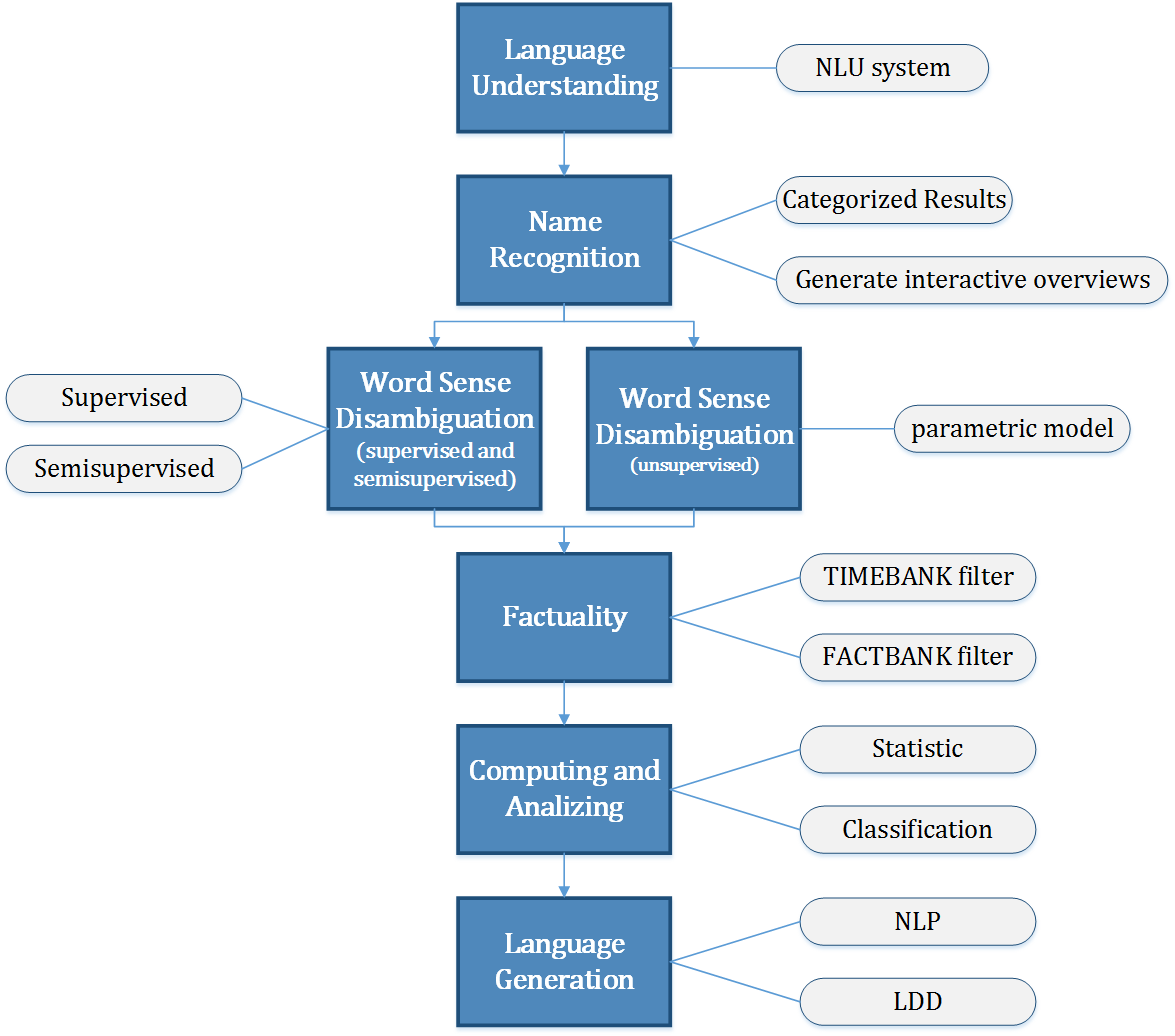
\includegraphics[width=1.8\columnwidth]{Union_Background_Chart_1}
	\end{center}
	\caption{The process of metadata creation.}
\end{figure*}

\subsubsection*{Language understanding}

Natural language understanding (NLU) is a subtopic of natural language processing in artificial intelligence that deals with machine reading comprehension, it's considered an AI-hard problem.

For a machine to understand language, it first has to develop a mental map of words, their meanings and interactions with other words. It needs to build a dictionary of words, and understand where they stand semantically and contextually, compared to other words in their dictionary. To achieve this, each word is mapped to a set of numbers in a high-dimensional space, which are called “word embeddings”. Similar words are close to each other in this number space, and dissimilar words are far apart. Some word embeddings encode mathematical properties such as addition and subtraction.

After the machine has learned word embeddings, the next problem to tackle is the ability to string words together appropriately in small, grammatically correct sentences which make sense. This is called language modeling. Language modeling is one part of quantifying how well the machine understands language.

For example, given a sentence “I am eating pasta for lunch.”, and a word “cars”, if the machine can tell you with high confidence whether or not the word is relevant to the sentence “cars” is related to this sentence with a probability 0.01 and I am pretty confident about it, then that indicates that the machine understands something about words and contexts.

An even simpler metric is to predict the next word in the sentence. Given a sentence, for each word in its dictionary the machine assigns a probability of the word’s likeliness to appear next in the sentence. For example: “I am eating (     ).” To fill in the blank, a good language model would likely give higher probabilities to all edibles like “pasta”, “apple”, or “chocolate”, and it would give lower probability to other words in the dictionary which are contextually irrelevant like “taxi”, “building”, or “music”.

When users search for a sentence, how does the program understand the certain inputs of text? We could build a natural language understanding (NLU) system, in which the system's rules for semantic interpretation are learnt automatically from training data, which uses a set of possible yes-no questions that can be applied to data items.
After that, it follows rules for selecting the best questions at any node on the basis of training data by using a method for pruning trees to prevent over-training.

\subsubsection*{Name Recognition}

If users search for the word "Turkey", the results could be a country or an animal. 
The meaning is totally different and definitely make users very confused if he or she is not very familiar with the word "Turkey". 

There are a lot of misunderstandings like this if users search some words which have multiply meanings. 
Sometimes, the results are fully unrelated and this situation is always annoying. 
That would be troublesome when we count frequency of certain words to rank them.

Therefore, it is significantly crucial for a program to totally understand what users want by name recognition in natural language processing, finally they can find out the results much quicker and will not be confused anymore.

The method to improve the problem above is "categorize the words based on different subjects, topic, or genres" by using online database and python program. 
Metadata is limited in digital libraries and web resources, try to enlarge them with meaningful, organized and desired categories \cite{Kules2006}.

Besides dealing with mutiple-meaning words, the most important part of name recognition is to recognize the special names and terms such as locations, people name, country, even company names and academic terms.
Therefore, it is better for search engine to know what user want and huge name corpus are necessary. 
Plus, this work also can assist previous work.

With above effort, users' exploration and overviews of information could be better supported. It will be very convenient to find the results we want and lower the possibility of misunderstandings if users are not very familiar with finding the appropriate result in specific fields.
\cite{TunThuraThet2010} Users don't need to filter the results which are ranked by browsing frequency popularity but can just obtain the information and relevance by clicking the specific categories and some reasonable choices.

Plus, creating some choices for users is also vital because this make the searching much more oragnized. 
For example, if there are a lot of subtitles such as abstract, introduction, method, or references in some standard research articles, try to make some choices so that the users can easily find out what they want. 
There are a lot of different standard articles in the world.
 Making a suitable choices if someone want to creat a personalzed search engine and interface. 

Also, users are able to choose multiply fields if the results include a lot of relevant fields. 
That's a big motivation for people to handle these problems. 

A lot of online services have done similar tasks before. 
Thus, creating and using an online databases or automated metadata creation are to be recommended. 
The reason is there are many advantages, including integrating with the other cloud services or scaling with what users need such as how to categorize the categories. 
It is beneficial for people who would like to create a convenient and personalized database or metadata.\\\\\\


\todo[inline]{A summary on list format can be motivated, but then each item need to be brief and you should not introduce anything new like UMLS in it.}

\subsubsection*{Factuality}

In the process of producing metadata, which should be the most precise information and representing the text, validity of such metadata must be checked. Therefore, tools for fact checks are developed based on linguistic techniques. 

The tool could detect facts and excludes authors' subjective opinions \cite{Agerri2014}. From the authors's perspective, the two main set of tools having such functions is TIMEBANK and FACTBANK. (yes, the authors used capitalized name)

TIMEBANK was first proposed in \cite{pustejovsky2003timebank}. 
The idea was based on that English language has different tenses which could be exploited as signals for fact check. 
An example below could help to clarify the ideas. Let's examine these sentences:

\begin{itemize}
	\item I will go to Chimei museum tomorrow.
	\item Chimei museum is near Tainan District.
	\item I was in UK in 2012.
\end{itemize}

The first sentence is simple future tense which implies something has never actually happened, the second sentence is simple present tense which can directly imply facts, and the last sentence is in simple past tense which is about something already happened (which is facts), but is no longer a fact right now, so such fact must be used with caution. 

The reason for introducing such tool is that even scientific research articles can be glittering with subjective comments, opinions or even assumption from authors \cite{schultze2000confessional}. In addition to TIMEBANK, many other tools can be another filter for fact extraction. \cite{Dave2003mining} Identify words, clauses and phrases that show emotional state of the authors. 

The choice in expression of facts could also be a helpful indicator to show whether authors are subjectively supporting a cause, an opinion and so on \cite{Wiebe2005}. Among these mentioned approaches, this paper highly favors creation a kind of thesaurus compiled of linguistic signaling for non-factually statements such as FACTBANK, which is built by \cite{Sauri2009}. 
Following example shows how subjective statements can be picked out.

\begin{itemize}
	\item Channelization would guarantee high flow velocity in rivers, flooding and consequent degradation of riparian community (1a).
	\item Funding agencies would be happy with big entrepreneurs, instead of small and medium enterprises (1b).
	\item Tolerance to dictatorship would has negative influences on anarchist movement (2a).
	\item Tolerance to dictatorship would doom anarchist movement (2b).
\end{itemize}

It is easy to find in statement (1a) is an absolute fact. 
Statement (1b) is however affected by emotional state of authors. 
After re-writing (1b) into: Funding agencies lend more money with lower interest rate to big entrepreneurs, instead of small 
and medium enterprises,sentence (1b) become a face-based statement. 
In another case, statement (2a) is a fact-based statement while in statement (2b), authors are stressing their dislike toward dictatorship.

Fact checks in language generation is a new field but many useful tools have been developed. Each of them has their own function and could complement each others. In the limit of this study, we are using both of TIMEBANK and FACTBANK together for fact check.


\subsection{API and search engine}
An API is short-hand of  application programming interface, which include components to define a process of communication and data processing on computer. 
It is necessary to create a search engine as we mentioned at the beginning of this report.
A good example of API is HAPI on Python. 
According to \cite{Kochanov201615}, HAPI is a library included in Python. 
As the library has a collection of defined process, it allow users and other parties (which could be robots or others users at other ends) to interact with each other.
Main functions of the HAPI have been including sending uploads, data filtration and other manipulation. 
The outcomes of such process can be formatted with variable forms. 
As described by \cite{Hedbrant20162206}, programming interface can include following systems:
\begin{itemize}
	\item SOAP: Simple Object Access Protocol
	\item REST: Representational State Transfer
	\item UDDI: Universal Description, Discovery, and Integration
	\item WSDL: Web Service Definition Language
\end{itemize}
	Other programing system can be included as well. 
	SOAP is among a field attracting many recent researches. 
	A good review about SOAP could be found from the work of \cite{Hsieh2009424}. 
	SOAP has important roles in field monitoring as handling a huge amount of data can be trouble some in many senses. 
	SOAP in conjunction with other programming techniques, such as distributed computing, are employed because it can solve 3 problems listed below:
	\begin{itemize}
		\item Is the system scalable: 
		There are systems that suitable for a fixed amount of data, but not functional when the need of expending data storage comes in place. 
		With such system, programmers will have to build another system. 
		That would be a waste of human resource, time and money.
		\item Is the system reliable: 
		In other words, can data be stored safely. 
		Many data obtained in field monitoring are expensive. 
		Therefore, it is important to make sure data will be always there whenever a need of retrieval arisen. 
		Also, the data may be retrieved, processed and formatted by many people involved in the system.
		A reliable system will not be broken down easily and foremost, data will be safely stored.
		\item Is the system accessible: 
		This matter can be put in two questions 1- When we need to use the data, is it hard to retrieve it from the system. 
		Do we need trained personal to do that job.
		And if we do, which level of training is necessary. 
		2- How many people can access the system. 
		
	\end{itemize}
	It is proven in many engineering projects, the application of SOAP can help overcome these problems, especially in term of increasing accessiblity.
	\subsubsection{Search engine}
	As mentioned above, creating a search engine is an example of API application. 
	In this section we feel the need to give an example of how to create search engine with API. 
	We found an inspirational example from the work of \cite{Noei2016135}. 
	Although the authors not just using SOAP, but also more advanced Object Access Protocol such as Java, it shows that OAP in general improve code and design. 
	Consequently, it saves time and effort in developing new program.
	The authors also offer EXAF (EXample Applications Finder) so that program developers can find other examples that fits their interest.
	
\newpage % Ends the current page and causes all figures and tables to be printed
	
	\section{Harvard citation}
	\label{Harvard}
	%%%%%%%%%%%%%%%%%%%%%%%%%%%%%%%%%%%%%%%%%%%%%%%%%%%%%%%%%%%%%%%%%%%
% Harvard Citation
% Year:
% 2017
% Team:
% RCPL
% Members: 
% Lewis Hsu, Paul Lin, Tam-Van Ngo
% Relative files:
% Appendix_Harvard_citation.tex
% Note:    
% Do not compile this file compile Main.tex to get the pdf file instead.
%%%%%%%%%%%%%%%%%%%%%%%%%%%%%%%%%%%%%%%%%%%%%%%%%%%%%%%%%%%%%%%%%%%

\subsection{Harvard Citation format}

“According to \cite{James2008}, Harvard citation format is also known as the APA style or, more colloquially, as the ‘name(date)’ system. This is because an author’s surname in the text is followed by the date of the publication in brackets, and entries in the reference list are listed alphabetically, starting with the name and the initials of the author(s) followed by the date of publication for each entry.

Structure: Last name, First initial. (Year published). Article Title. Journal, [online] Volume(Issue), pages. Available at: URL [Accessed Day Mo. Year].

Example: LRaina, S. (2015). Establishing Correlation Between Genetics and Nonresponse. Journal of Postgraduate Medicine, [online] Volume 61(2), p. 148. Available at: http://www.proquest.com/products-services/ProQuest-Research-Library.html [Accessed 8 Apr. 2015].

For further references see \href{http://www.citethisforme.com/harvard-referencing}{harvard-referencing}


		
	%%%%%%%%%%%%%%%%%%%%%%%%%%%%%%%%%%%%%%%%%%%%%%%%%%%%%%%%%%%%%%%%%%%
	% References
	% Using Mendeley Desktop with library.bib
	%%%%%%%%%%%%%%%%%%%%%%%%%%%%%%%%%%%%%%%%%%%%%%%%%%%%%%%%%%%%%%%%%%%		
	\bibliographystyle{agsm_nurl}
	\bibliography{library}	
	\clearpage 
\end{document}  
